%%
%% This is file `docultexmm.tex', 
%% Documentation for siam multimedia macros for use with LaTeX 2e
%% 
%% December 19, 2013
%%
%% Version 1.0.1
%% 
%% You are not allowed to change this file. 
%% 
%% You are allowed to distribute this file under the condition that 
%% it is distributed together with all of the files in the siam macro 
%% distribution. These are:
%%
%%  siamltexmm.cls (this file)
%%  siam11.clo   (required size option for 11pt papers)
%%  subeqn.clo   (allows equation numbers with lettered subelements)
%%  siam.bst     (bibliographic style file for BibTeX)
%%  docultexmm.tex (documentation file)
%%
%% If you receive only some of these files from someone, please contact: 
%% multimedia@siam.org  
%% 
%% You are not allowed to distribute this file alone. You are not 
%% allowed to take money for the distribution or use of either this 
%% file or a changed version, except for a nominal charge for copying 
%% etc.
%%
%% \CharacterTable
%%  {Upper-case    \A\B\C\D\E\F\G\H\I\J\K\L\M\N\O\P\Q\R\S\T\U\V\W\X\Y\Z
%%   Lower-case    \a\b\c\d\e\f\g\h\i\j\k\l\m\n\o\p\q\r\s\t\u\v\w\x\y\z
%%   Digits        \0\1\2\3\4\5\6\7\8\9
%%   Exclamation   \!     Double quote  \"     Hash (number) \#
%%   Dollar        \$     Percent       \%     Ampersand     \&
%%   Acute accent  \'     Left paren    \(     Right paren   \)
%%   Asterisk      \*     Plus          \+     Comma         \,
%%   Minus         \-     Point         \.     Solidus       \/
%%   Colon         \:     Semicolon     \;     Less than     \<
%%   Equals        \=     Greater than  \>     Question mark \?
%%   Commercial at \@     Left bracket  \[     Backslash     \\
%%   Right bracket \]     Circumflex    \^     Underscore    \_
%%   Grave accent  \`     Left brace    \{     Vertical bar  \|
%%   Right brace   \}     Tilde         \~}

\documentclass[final,leqno,onefignum,onetabnum]{siamltexmm}

\usepackage{amsmath}
\usepackage{amsfonts}

\usepackage{epsfig}

\title{Data-driven Reduction of Multiscale Stochastic Dynamical Systems \thanks{This work was
supported by ....}} 

\author{Carmeline J. Dsilva\footnotemark[2] \and Ronen Talmon\footnotemark[3] \and C. William Gear\footnotemark[2] \and Ronald R. Coifman\footnotemark[3] \and Ioannis G. Kevrekidis\footnotemark[2]\ \footnotemark[4]}

\begin{document}
\maketitle
\newcommand{\slugmaster}{%
\slugger{siads}{xxxx}{xx}{x}{x--x}}%slugger should be set to juq, siads, sifin, or siims

\renewcommand{\thefootnote}{\fnsymbol{footnote}}

\footnotetext[2]{Department of Chemical and Biological Engineering, Princeton University, Princeton, New Jersey, 08544, USA}
\footnotetext[3]{Department of Mathematics, Yale University, New Haven, Connecticut, 06520, USA}
\footnotetext[4]{Program in Applied and Computational Mathematics, Princeton University, Princeton, New Jersey, 08544, USA}

\renewcommand{\thefootnote}{\arabic{footnote}}

\begin{abstract}

\end{abstract}

\begin{keywords}\end{keywords}

\begin{AMS}
37M10, 62-07
\end{AMS}

\pagestyle{myheadings}
\thispagestyle{plain}
\markboth{C.~J. DSILVA {\it ET AL}}{DATA-DRIVEN REDUCTION OF SDES}


\section{Introduction}

\begin{itemize}

\item
Bridge/connect between data mining/analysis and dynamical systems

\begin{itemize}

\item
Main idea and scope: analyze stochastic dynamical systems using data-driven methods.

\begin{itemize}

\item
Reduction in fast-slow systems using manifold learning

\end{itemize}

\end{itemize}
\item
We cannot use off-the-shelf data-driven methods because they are typically based on metrics and geometry and are not informed (take into account) the dynamics and time.

\item
Our contribution:

\begin{itemize}

\item
We show how to use data analysis methods that are typically applied to data sets for analyzing data collected as a time series from a dynamical system. In particular, we ``propose" a data-driven (graph-based) method for recovering the slow variable of reducible systems.

\item
The method is based mostly on local analysis that combines geometry and dynamics.

\item
We offer rigorous analysis for the method that gives the conditions (for our method to successfully recover the ``right" slow variables), intuition.

\end{itemize}

\end{itemize}

\subsection{Multiscale SDEs}

We consider the following two-scale SDE, 
\begin{equation} \label{eq:general_SDE}
\begin{aligned}
dx_i &= a_i(\vec{x}) dt + dW_i, & \: 1 \le i \le m \\
dx_i &= \frac{a_i(\vec{x})}{\epsilon} dt + \frac{1}{\sqrt{\epsilon}} dW_i , & \: m+1 \le i \le n
\end{aligned}
\end{equation}
where $W_i$ are independent standard Brownian motions, $\vec{x}  = \begin{bmatrix} x_1 & \cdots & x_n \end{bmatrix}^T \in \mathbb{R}^n$, and $\epsilon \ll 1$.
%
Therefore, \eqref{eq:general_SDE} defines an $n$-dimensional stochastic system with $m$ slow variables and $n-m$ fast variables. 
%
We would like to note that the ratio of the drift and diffusion terms is essential, as we need the square of the diffusivity to be of the same order as the drift.
%
If the diffusivity is too large, then, as $\epsilon \rightarrow 0$, the equilibrium measure will be unbounded.
%
Conversely, if the diffusivity is too small, the equilibrium measure will go to 0 as $\epsilon \rightarrow 0$.

Assuming that the functions $a_i$ are bounded and Lipschitz, and that we can find functions $\kappa_i(T)$, $1 \le i \le m$, such that
\begin{equation}
\mathbb{E} \left| \frac{1}{T} \int_t^{t + T} a_i(x_1, \dots, x_m, x_{m+1}(s), \dots, x_n(s)) ds - \overline{a} (x_1, \dots, x_m) \right| < \kappa_i (T), 
\end{equation}
with $\kappa_i(T) \rightarrow 0 $ as $T \rightarrow \infty$, then the averaging principle \cite{...} states that we can write an effective SDE in {\em only} the slow variables $x_1, \dots, x_m$. 

We will consider observing the the SDE in \eqref{eq:general_SDE} through a deterministic (perhaps nonlinear) function $\mathbf{f}: \mathbb{R}^n \mapsto \mathbb{R}^d$, where $d \ge n$ and the image of $\mathbf{f}$ is an $n$-dimensional manifold in $\mathbb{R}^d$. 
%
We require the $\mathbf{g} = \mathbf{f}^{-1}$ to be well-defined, and both $\mathbf{f}$ and $\mathbf{g}$ to be continuously differentiable to fourth order. 
%
Our goal is to recover a parameterization of the data which respects/is one-to-one with the slow variables $x_1, \dots, x_m$  from observations of $\mathbf{f}(\vec{x})$ using data-driven techniques. 

\section{Local Invariant Metrics}

To locally recover the slow variables, we need to build a metric that is invariant to the fast variables. 
%
Typically, this is done by averaging out the fast variables. 
%
We propose to do this using the Mahalanobis distance, which is a local PCA-type approach that inverts the local covariance matrix of the data, thereby creating a space with normalized diffusion terms.
%
It can be shown \cite{...} that the Mahalanobis distance, $\| \cdot \|_M$, locally approximates: 
\begin{equation} \label{eq:mahalanobis}
\| \mathbf{f}(\vec{x}_2) - \mathbf{f}(\vec{x}_1) \|^2_M = \| \vec{z}_2 - \vec{z}_1 \|^2_2 + \mathcal{O}(\| \mathbf{f}(\vec{x}_2) - \mathbf{f}(\vec{x}_1) \|^4_2)
\end{equation}
where the components of $\vec{z}$ are sampled from a stochastic process with uncoupled noise with unit variance,
i.e., $\vec{z} = \begin{bmatrix} z_1 & z_2 & \cdots & z_n \end{bmatrix}^T \in \mathbb{R}^n$, where $z_1, \dots, z_n$ are governed by the following SDEs:
\begin{equation} \label{eq:NIV_formulation}
dz_i = b_i(\vec{z}) dt + dW_i
\end{equation}

To relate this metric with our SDE formulation, we first define the vector $\vec{e} \in \mathbb{R}^n$ with
\begin{equation}
\begin{aligned}
e_i =& 1, \: & 1 \le i \le m \\
e_i =& \epsilon, \: & m+1 \le i \le n
\end{aligned}
\end{equation}
%
We then consider the transformation
\begin{equation} \label{eq:general_rescale}
x_i = \frac{z_i}{\sqrt{e_i}}
\end{equation}
so that \eqref{eq:general_SDE} now becomes
\begin{equation} 
\begin{aligned}
dz_i &= a_i(\vec{z}) dt + dW_i, & \: 1 \le i \le m \\
dz_i &= \frac{a_i(\vec{z})}{\sqrt{\epsilon}} dt + dW_i , & \: m+1 \le i \le n
\end{aligned}
\end{equation}
%
From \eqref{eq:general_rescale}, we can see 
\begin{equation}
\| \vec{z}_2 - \vec{z}_1 \|^2_2 = \sum_{i=1}^n \left( z_{2,i} - z_{1,i} \right)^2 = \sum_{i=1}^n e_i \left( x_{2,i} - x_{1,i} \right)^2
\end{equation}
%
Remarkably, this metric induces two important features. 
%
One, rescaling the data so that all variables have unit diffusion terms means that fast variables are collapsed and become $\sqrt{\epsilon}$ small, as observed in the second term in the right hand side. 
%
Two, the righthandside of \eqref{eq:mahalanobis} is invariant (to fourth order) to the function $\mathbf{f}$ and allows for the approximation of the Euclidean distance between samples of the slow variables in the ``decoupled" SDE space.


\section{Diffusion Maps for Global Parameterization}

Our goal is to extract a {\em global} parameterization of the data that respects the slow variables. 
%
We will use diffusion maps, a kernel-based manifold learning technique, to extract a global parameterization using the local distances that we described in the previous section. 
%
Given data $\vec{v}_1, \dots, \vec{v}_N \in \mathbb{R}^d$, we first construct the matrix $W \in \mathbb{R}^{N \times N}$, where 
\begin{equation} \label{eq:dmaps_kernel}
W_{ij} = \exp \left( -\frac{\|\vec{v}_i - \vec{v}_j \|^2}{\sigma_{kernel}^2} \right)
\end{equation}
where $\| \cdot \|$ denotes the appropriate norm (in our case, the Mahalanobis distance \eqref{eq:mahalanobis}), and $\sigma_{kernel}$ is the kernel scale and denotes a characteristic distance within the data set. 
%
We then construct the diagonal matrix $D \in \mathbb{R}^{N \times N}$, with 
\begin{equation}
D_{ii} = \sum_{j=1}^N W_{ij}
\end{equation}
%
We compute the eigenvalues $\lambda_0, \dots, \lambda_{N-1}$ and eigenvalues $\phi_0, \dots, \phi_{N-1}$ of the matrix $A = D^{-1}W$, and order them such that $|\lambda_0| \ge |\lambda_1| \ge \dots \ge |\lambda_{N-1}|$. 
%
$\phi_0$ is a constant trivial eigenvector; the next few eigenvectors give a parameterization/embedding coordinates for the data (modulo higher harmonics which characterize the same direction in the data). 

\section{Analysis}

\begin{figure}[t]
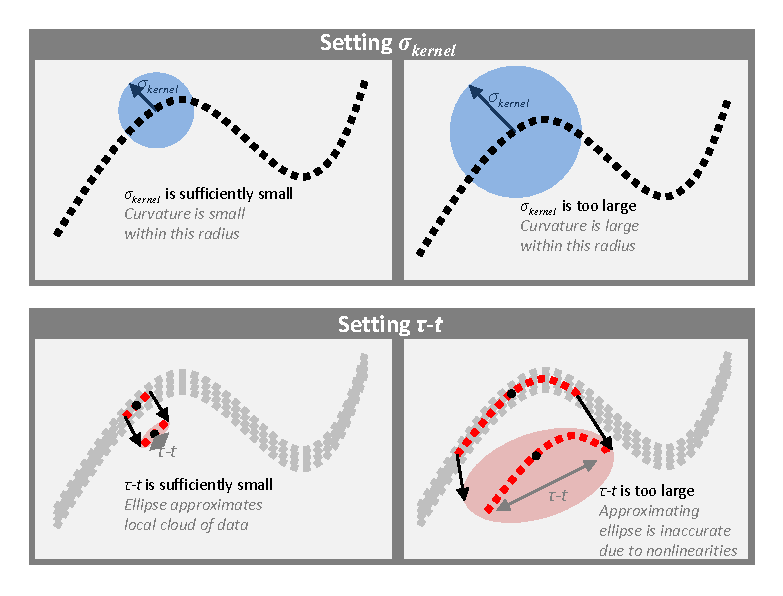
\epsfig{width=\textwidth, file=schematic.eps}
\caption{Illustration of how to choose $\delta t$ and $\sigma_{kernel}$ appropriately. The data shows the evolution of the ``fast'' variable at a fixed value of the ``slow'' variable.  We must choose both parameters so that the curvature effects and other nonlinearities are negligable. }
\label{fig:schematic}
\end{figure}

Our approximation of the pairwise distances will rely on the Taylor expansion of the measurement function $\mathbf{f}$. 
%
We will then {\em empirically} estimate the first-order term in this expansion using simulation bursts to estimate the local covariance.  
%
Accordingly, we will address the accuracy of our method from two standpoints: (1) the accuracy of the Taylor expansion, and (2) the accuracy of the covariance estimation (see Figure~\ref{fig:schematic}).
%
We will present both analytical results for the error bounds, as well as an empirical methodology to set the appropriate parameters for our method to accurately recover the intrinsic slow variable(s). 

%TODO: change strip to look different than other data

\subsection{Error analysis of the Mahalanobis distance}

We want to calculate the distance $\|\vec{z}_2 - \vec{z}_1\|_2$ in terms of the observations $\vec{y} = \mathbf{f}(\vec{x})$. 
%
Let $\mathbf{g} = \mathbf{f}^{-1}: \mathbb{R}^d \mapsto \mathbb{R}^n$, such that
\begin{equation} \label{eq:variable_rescaling}
\sqrt{e_i} g_i(\vec{y}) = \sqrt{e_i} x_i = z_i
\end{equation}
%
Let $\vec{y}_1 = \mathbf{f}(\vec{x}_1)$, and $\vec{y}_2 = \mathbf{f}(\vec{x}_2)$.
%
By Taylor expansion of $\mathbf{g}(y)$ around $\vec{y}_1$ and $\vec{y}_2$ and averaging, and then substituting the relationships in \eqref{eq:variable_rescaling}, we obtain 
%
{\small
\begin{equation} \label{eq:distance_taylor_expansion}
\begin{aligned}
&\| \vec{z}_2 - \vec{z}_1 \|^2_2 = \\
& \frac{1}{2} \sum_{i=1}^n \sum_{jk=1}^d e_i \left( \left. \frac{\partial g_i}{\partial y_j} \right|_{\vec{y}_1} \left. \frac{\partial g_i}{\partial y_k} \right|_{\vec{y}_1} + \left. \frac{\partial g_i}{\partial y_j} \right|_{\vec{y}_2} \left. \frac{\partial g_i}{\partial y_k } \right|_{\vec{y}_2} \right) (y_{2,j} - y_{1,j}) (y_{2,k} - y_{1,k}) \\
& + \frac{1}{2} \sum_{i=1}^n \sum_{jkl=1}^{d} e_i \left( \left. \frac{\partial g_i}{\partial y_j} \right|_{\vec{y}_1} \left. \frac{\partial^2 g_i}{\partial y_k \partial y_l} \right|_{\vec{y}_1} - \left. \frac{\partial g_i}{\partial y_j} \right|_{\vec{y}_2} \left. \frac{\partial^2 g_i}{\partial y_k \partial y_l} \right|_{\vec{y}_2} \right) (y_{2,j} - y_{1,j})  (y_{2,k} - y_{1,k})(y_{2,l} - y_{1,l}) \\
& + \frac{1}{8} \sum_{i=1}^n \sum_{jklm=1}^d  e_i \left( \left. \frac{\partial^2 g_i}{\partial y_j \partial y_k} \right|_{\vec{y}_1} \left. \frac{\partial^2 g_i}{\partial y_l \partial y_m} \right|_{\vec{y}_1} + \left. \frac{\partial^2 g_i}{\partial y_j \partial y_k} \right|_{\vec{y}_2} \left. \frac{\partial^2 g_i}{\partial y_l \partial y_m} \right|_{\vec{y}_2} \right) (y_{2,j} - y_{1,j})  (y_{2,k} - y_{1,k})(y_{2,l} - y_{1,l})(y_{2,m} - y_{1,m}) \\
& + \frac{1}{6} \sum_{i=1}^n \sum_{jklm=1}^d e_i \left( \left. \frac{\partial g_i}{\partial y_j} \right|_{\vec{y}_1} \left. \frac{\partial^3 g_i}{ \partial y_k \partial y_l \partial y_m} \right|_{\vec{y}_1} + \left. \frac{\partial g_i}{\partial y_j} \right|_{\vec{y}_2} \left. \frac{\partial^3 g_i}{ \partial y_k \partial y_l \partial y_m} \right|_{\vec{y}_2} \right) (y_{2,j} - y_{1,j})  (y_{2,k} - y_{1,k})(y_{2,l} - y_{1,l})(y_{2,m} - y_{1,m}) \\
& + \mathcal{O} (\|\vec{y}_1 - \vec{y}_2 \|^6 ),
\end{aligned}
\end{equation}
}
assuming that terms involving the differences of derivatives evaluated at $\vec{y}_1$ and $\vec{y}_2$ are $\mathcal{O}(\|\vec{y}_2 - \vec{y}_1\|)$.
%
In general, we do not have access to $\mathbf{f}$, $\mathbf{g}$, or any of its derivatives.
%
However, we note that 
\begin{equation}
\begin{aligned}
\frac{1}{2} \sum_{i=1}^n \sum_{jk=1}^d e_i \left( \left. \frac{\partial g_i}{\partial y_j} \right|_{\vec{y}_1} \left. \frac{\partial g_i}{\partial y_k} \right|_{\vec{y}_1} + \left. \frac{\partial g_i}{\partial y_j} \right|_{\vec{y}_2} \left. \frac{\partial g_i}{\partial y_k } \right|_{\vec{y}_2} \right) (y_{2,j} - y_{1,j}) (y_{2,k} - y_{1,k}) \\
= \frac{1}{2} (\vec{y}_2 - \vec{y}_1)^T \left( C^{\dagger}(\vec{y}_1) + C^{\dagger}(\vec{y}_2) \right) (\vec{y}_2 - \vec{y}_1)
\end{aligned}
\end{equation}
%
where $C(\vec{y})$ is the local covariance of observed stochastic process at $\vec{y}$, which we can empirically estimate from data (this will be discussed in a subsequent section), and $C^{\dagger}(\vec{y})$ denotes the rank-$n$ Moose-Penrose pseudoinverse (since, in general, $d \ge n$).
%
Therefore, we choose to truncate the distance approximation in \eqref{eq:distance_taylor_expansion} at the first order term.
%
We call this distance the Mahalanobis distance \footnote{We would like to note that the Mahalanobis distance is traditionally defined for a fixed covariance matrix. However, following \cite{...}, we will define our Mahalanobis distance locally, using the local covariance at each point.}, 
\begin{equation} \label{eq:mahalanobis_distance}
 \| \vec{y}_2 - \vec{y}_1 \|^2_M = 
 \frac{1}{2} (\vec{y}_2 - \vec{y}_1)^T \left( C^{\dagger}(\vec{y}_1) + C^{\dagger}(\vec{y}_2) \right) (\vec{y}_2 - \vec{y}_1)
 \end{equation}
%
We define the error incurred by using the Mahalanobis distance to approximate the true distance between the points as
\begin{equation} \label{eq:mahanaobis_error}
e_M(\vec{y}_1, \vec{y}_2) \equiv \| \vec{z}_2 - \vec{z}_1 \|^2_2 - \| \vec{y}_2 - \vec{y}_1 \|^2_M 
\end{equation}

The parameter $\sigma_{kernel}$ in the DMAPS calculation determines how much $e_M$ contributes to our overall analysis. 
%
From \eqref{eq:dmaps_kernel}, we can see that distances which are greater than $\sigma_{kernel}$ are ``not important'' in the computation, as their weight goes to 0 because of the exponential kernel. 
%
Therefore, we want to choose $\sigma_{kernel}^2$ on the order of $\|\vec{y}_2 - \vec{y}_1\|^2$ in a regime where $e_M \ll \|\vec{y}_2 - \vec{y}_1\|^2$. 
%
This will ensure that the errors in the Mahalanobis distance approximation do not contribute greatly to our overall analysis. 

\subsection{Error analysis of the covariance estimation}

To compute the Mahalanobis distance in \eqref{eq:mahalanobis_distance}, we require $C$, the local covariance of the observed stochastic process. 
%
Therefore, we would like to estimate the local covariance at a point $\vec{x}_t$. 

We know that, for a stochastic process following \eqref{eq:general_SDE} and observed through a function $\mathbf{f}$, the covariance $C$ is given by 
\begin{equation}
C_{i_1 i_2}(\vec{x}_t) = 
\sum_{j=1}^n \frac{1}{e_j} \left. \frac{\partial f_{i_1}}{\partial x_j} \right|_{\vec{x}_t} \left. \frac{\partial f_{i_2}}{\partial x_j} \right|_{\vec{x}_t} 
\end{equation}
%
We will use local simulation bursts to estimate the local covariance,
\begin{equation} \label{eq:est_cov}
\hat{C}_{i_1 i_2}(\vec{x}_t, \delta t) =
\frac{1}{\delta t} \left( \mathbb{E} \left[ f_1(\vec{x}_{t + \delta t}) f_2(\vec{x}_{t + \delta t}) \right] 
- \mathbb{E} \left[ f_1(\vec{x}_{t + \delta t}) \right] \mathbb{E} \left[ f_2(\vec{x}_{t + \delta t}) \right] \right)
\end{equation}
%
where $\delta t > 0$ is the length of the simulation burst. 
%
For the general SDE formulation outlined in \eqref{eq:general_SDE}, the estimated covariance $\hat{C}$ is 
\begin{equation}\label{eq:estimated_cov}
\begin{aligned}
\hat{C}_{i_1 i_2}(\vec{x}_t, \delta t) 
=& 
\sum_{j=1}^n  \frac{1}{e_j} \left. \frac{\partial f_{i_1}}{\partial x_j} \right|_{\vec{x}_t} \left. \frac{\partial f_{i_2}}{\partial x_j} \right|_{\vec{x}_t} \\
&+ \frac{1}{\delta t} \sum_{j,k,l=1}^n \frac{1}{\sqrt{e_j e_k e_l}} \left. \frac{\partial f_{i_1}}{\partial x_j} \right|_{\vec{x}_t} \mathbb{E} \left[ \left( \int_t^{t + \delta t} dW_{s,j} \right) \left( \int_t^{t+\delta t} \int_t^{s_2} \left. \frac{\partial^2 f_{i_2}}{\partial x_k \partial x_l} \right|_{\vec{x}_{s_1}} dW_{s_1, k} dW_{s_2, l} \right) \right] \\
&+ \frac{1}{\delta t}  \sum_{j,k,l=1}^n \frac{1}{\sqrt{e_j e_k e_l}} \left. \frac{\partial f_{i_2}}{\partial x_j} \right|_{\vec{x}_t} \mathbb{E} \left[ \left( \int_t^{t + \delta t} dW_{s,j} \right) \left( \int_t^{t+\delta t} \int_t^{s_2} \left. \frac{\partial^2 f_{i_1}}{\partial x_k \partial x_l} \right|_{\vec{x}_{s_1}} dW_{s_1, k} dW_{s_2, l} \right) \right] \\
&+ \mathcal{O} (\delta t)
\end{aligned}
\end{equation}

However, for the specific case when $\mathbf{f}$ is linear, the $\mathcal{O}(\sqrt{\delta t})$ drop out, and we must consider higher-order terms. 
%
In this case, 
%
\begin{equation} \label{eq:estimated_cov_linear_f}
\begin{aligned}
\hat{C}_{i_1 i_2}(\vec{x}_t, \delta t) 
=& 
\sum_{j=1}^n  \frac{1}{e_j} \frac{\partial f_{i_1}}{\partial x_j} \frac{\partial f_{i_2}}{\partial x_j} \\
&+ \frac{1}{\delta t} \sum_{j,k,l=1}^n \frac{1}{e_l \sqrt{e_j e_k}} \frac{\partial f_{i_1}}{\partial x_j} \mathbb{E} \left[ \left( \int_t^{t + \delta t} dW_{s,j} \right)\left( \int_t^{t+\delta t} \int_t^{s_2}  \frac{\partial f_{i_2}}{\partial x_l} \left. \frac{\partial a_l(\vec{x})}{\partial x_k} \right|_{\vec{x}_{s_1}} dW_{s_1, k} ds_2 \right) \right]\\
&+ \frac{1}{\delta t} \sum_{j,k,l=1}^n \frac{1}{e_l \sqrt{e_j e_k}} \frac{\partial f_{i_2}}{\partial x_j}  \mathbb{E} \left[ \left( \int_t^{t + \delta t} dW_{s,j} \right)\left( \int_t^{t+\delta t} \int_t^{s_2}  \frac{\partial f_{i_1}}{\partial x_l} \left. \frac{\partial a_l(\vec{x})}{\partial x_k} \right|_{\vec{x}_{s_1}} dW_{s_1, k} ds_2 \right) \right]\\
&+ \mathcal{O} (\delta t^{3/2})
\end{aligned}
\end{equation}
%
For both cases, we define the error in the covariance estimation as
%
\begin{equation} \label{eq:cov_error}
\begin{aligned}
e_C (\vec{x}_t, \delta t) \equiv \hat{C} (\vec{x}_t, \delta t)  - C(\vec{x}_t) 
\end{aligned}
\end{equation}

In practice, we will compute $\hat{C}$ using \eqref{eq:est_cov} by running many simulations of length $\delta t$ starting at point $\vec{x}_t$, and using the sample average to approximate the expected values. 
%
We want to set $\delta t$ such that $\|e_C \| \ll \|C \|$. 

\section{Results}

For illustrative purposes, we will consider the following two-dimensional SDE as a specific example of \eqref{eq:general_SDE}. 
\begin{equation} \label{eq:specific_SDE}
\begin{aligned}
dx_1 &=& adt &+& dW_1\\
dx_2 &=& -\frac{x_2}{\epsilon} dt &+& \frac{1}{\sqrt{\epsilon}} dW_2
\end{aligned}
\end{equation}
%
where $a$ is a constant of order 1. 
%
So $x_1$ is the slow variable, and $x_2$ is a fast noise whose equilibrium measure is bounded and $\mathcal{O}(1)$.
%
Figure~\ref{fig:initial_data} shows data simulated from this SDE, colored by time.
%
We would like to recover a parameterization of this data that is one-to-one with $x_1$ (the slow variable) using data-driven techniques.

\begin{figure}[t]
\centering
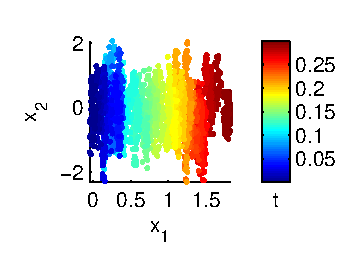
\epsfig{width=0.5\textwidth, file=data_init.eps}
\caption{Data, simulated from \eqref{eq:specific_SDE} with $a=3$ and $\epsilon = 10^{-3}$, for $3000$ timesteps with $dt = 10^{-4}$. The data are colored by time.}
\label{fig:initial_data}
\end{figure}

\subsection{Linear functions} \label{subsec:linear_example}

In the first example, our observation function $\mathbf{f}$ will be the identity function,
%
\begin{equation}
\begin{aligned}
\begin{bmatrix}
y_1 \\ y_2
\end{bmatrix} &=&
\mathbf{f}(\vec{x}) &=& 
\begin{bmatrix} x_1 \\ x_2 \end{bmatrix} \\
\mathbf{g}(\vec{y}) &=& \mathbf{f}^{-1} (\vec{y}) &=& \begin{bmatrix} y_1 \\ y_2 \end{bmatrix}
\end{aligned}
\end{equation}
%
For this example, the fast and slow variables remain uncoupled. 
%
In this case, $e_M = 0$, as the second- and higher-order derivatives of $\mathbf{g}$ are all 0. 

For this example, the analytical covariance is
 \begin{equation} \label{eq:cov_linear_example}
C(\vec{x}_t) = 
\begin{bmatrix}
1 & 0 \\
0 & \frac{1}{\epsilon}
\end{bmatrix}
\end{equation}

\subsubsection{NIVs versus DMAPS}

We first want to demonstrate the utility of using the Mahalanobis distance compared to the typical Euclidean distance. 
%
We compute the first (nontrivial) DMAPS coordinate using the data in Figure~\ref{fig:initial_data}, using both the Mahalanobis distance and the Euclidean distance in \eqref{eq:dmaps_kernel}.  
%
The results are shown in Figure~\ref{fig:NIV_versus_DMAPS}.
%
Using the Mahalanobis distance allows us to accurately recover the slow variable (the coloring in Figure~\ref{fig:NIV_versus_DMAPS}(a) is consistent with the coloring in Figure~\ref{fig:initial_data}). 
%
In contrast, using the Euclidean distance does not allow us recover the slow variable using DMAPS. 

\begin{figure}[t]
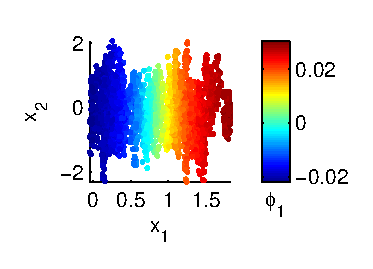
\epsfig{width=0.5\textwidth, file=data_linear_NIV.eps}
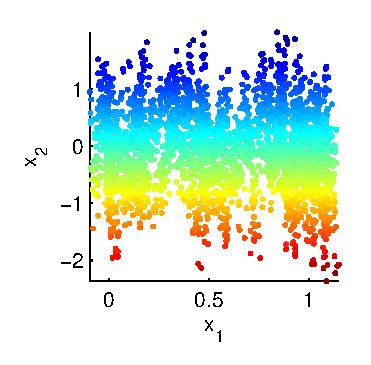
\epsfig{width=0.5\textwidth, file=data_linear_DMAPS.eps}
\caption{Comparison of using the Mahalanobis distance and the Euclidean distance. (a) The data from Figure~\ref{fig:initial_data}, colored by the first DMAPS coordinate when using the Mahalanobis distance in the DMAPS kernel. (b) The data from Figure~\ref{fig:initial_data}, colored by the first DMAPS coordinate when using the Euclidean distance in the DMAPS kernel. Note that we do {\em not} recover the slow variable.}
\label{fig:NIV_versus_DMAPS}
\end{figure}

\subsubsection{Errors in covariance estimation}

From \eqref{eq:estimated_cov_linear_f}, we calculate
\begin{equation}
\begin{aligned}
e_{C, 11}(\vec{x}_t, \delta t) =& \mathcal{O} (\delta t^{3/2}) \\
e_{C, 12}(\vec{x}_t, \delta t) =&  -\frac{1}{\delta t \epsilon^{3/2}} \mathbb{E} \left[ \left( \int_t^{t + \delta t} dW_{s,1} \right)\left( \int_t^{t+\delta t} \int_t^{s_2}  dW_{s_1, 2} ds_2 \right) \right] + \mathcal{O} (\delta t^{3/2})\\
e_{C, 21}(\vec{x}_t, \delta t) =& -\frac{1}{\delta t \epsilon^{3/2}} \mathbb{E} \left[ \left( \int_t^{t + \delta t} dW_{s,1} \right)\left( \int_t^{t+\delta t} \int_t^{s_2}  dW_{s_1, 2} ds_2 \right) \right] + \mathcal{O} (\delta t^{3/2})\\
e_{C, 22}(\vec{x}_t, \delta t) =& -\frac{2}{\delta t \epsilon^2} \mathbb{E} \left[ \left( \int_t^{t + \delta t} dW_{s,2} \right)\left( \int_t^{t+\delta t} \int_t^{s_2}  dW_{s_1, 2} ds_2 \right) \right] + \mathcal{O} (\delta t^{3/2}) 
\end{aligned}
\end{equation}
%
Therefore, $\|e_C \| = \mathcal{O}\left(\frac{\delta t}{\epsilon^2} \right)$, and from \eqref{eq:cov_linear_example}, $\| C \| = \mathcal{O} \left( \frac{1}{\epsilon} \right)$. 
%
These terms are shown in Figure~\ref{fig:cov_error}(a). 
%
We would like to choose $\delta t$ in a regime where $\|e_c \| \ll \| C\|$, so that the errors in the estimated covariance are small. 

We can find such a regime empirically when we do not know the functions $\mathbf{f}$ or $\mathbf{g}$. 
%
We can estimate the covaraince for several values of $\delta t$. 
%
This will provide an estimate of $\hat{C} = C + e_C$ as a function of $\delta t$.
%
From Figure~\ref{fig:cov_error}(a), we can see that there should be a kink in the plot of $\| \hat{C} \|$ versus $\delta t$ when $\| e_C \|$ becomes larger than $\|C\|$. 
%
Figure~\ref{fig:cov_error}(b) shows the empirical $\| \hat{C} \|$ as a function of $\delta t$, and the kink in this curve is consistent with the crossover point in Figure~\ref{fig:cov_error}(a). 

\begin{figure}[t]
\epsfig{width=0.5\textwidth, file=C_dt_analytical_linear.eps}
\epsfig{width=0.5\textwidth, file=C_dt_linear.eps}
%\epsfig{width=0.5\textwidth, file=data_linear_NIV_smalldt.eps}
\caption{Errors in covariance estimation for linear example. (a) The analytical expressions for the contributions to the covariance for the example in Section~\ref{subsec:linear_example} as a function of $\delta t$. (b) The average estimated covariance $\| \hat{C} \|$ as a function of $\delta t$. The average is computed over $10$ test points and using $50$ sample points to estimate the covariance.}
\label{fig:cov_error}
\end{figure}

\subsubsection{Recovery of fast variable}

Note that, for this linear example, $e_C$ is essentially a constant a diagonal matrix (the $e_{C,22} = \mathcal{O}(\frac{\delta t}{\epsilon^2})$ term dominates). 
%
Therefore, taking $\delta t$ ``too large'' will not lead to nonlinear effect or mixing of the fast and slow variables. %
Rather, changing $\delta t$, will only affect the ``perceived'' timescales of the fast/slow. 
%
Figure~\ref{fig:recover_fast} shows results for three different values of $\delta t$ (the corresponding values are indicated by the dashed lines on Figure~\ref{fig:cov_error}). 
%
When the time scale of the simulation burst used to estimate the local covariance (indicated by the red clouds in the top row of figures) is smaller than that of the equilibration time of the fast variable, the estimated covariance is constant and the fast variable is collapsed significantly relative to the slow variable.
%
This means that the fast variable is recovered {\em very} far down in the DMAPS eigenvectors; the left two columns show that, for this example, the fast variable is recovered as $\phi_{10}$.
%
However, if the time scale of the burst is {\em longer} than the saturation time of the fast variable, the estimated covariance changes: the variance in the slow direction continues to grow, while the variance in the fast direction is fixed.
%
This means that the collapse of the fast variable is less pronounced relative to the slow variable, and the fast variable is recovered in a higher eigenvector; the right column shows that, when the burst is now longer than the equilibration time, the fast variable appears higher in the eigenvalue spectrum and is recovered as $\phi_6$.

\begin{figure}[t]
\epsfig{width=0.3\textwidth, file=data_linear_burst1.eps}
\epsfig{width=0.3\textwidth, file=data_linear_burst2.eps}
\epsfig{width=0.3\textwidth, file=data_linear_burst3.eps}

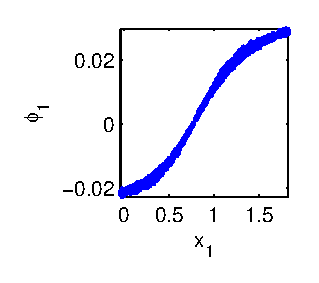
\epsfig{width=0.3\textwidth, file=data_linear_slow1.eps}
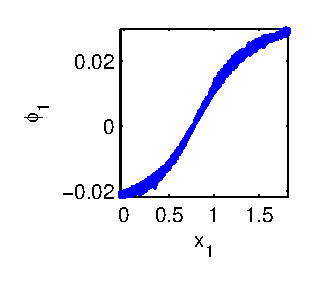
\epsfig{width=0.3\textwidth, file=data_linear_slow2.eps}
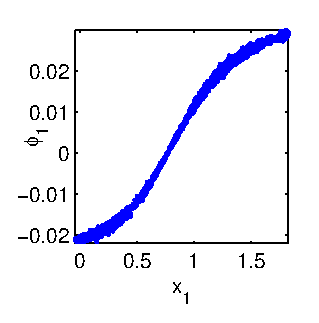
\epsfig{width=0.3\textwidth, file=data_linear_slow3.eps}

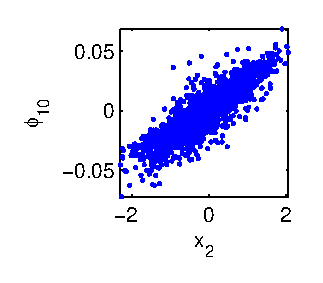
\epsfig{width=0.3\textwidth, file=data_linear_fast1.eps}
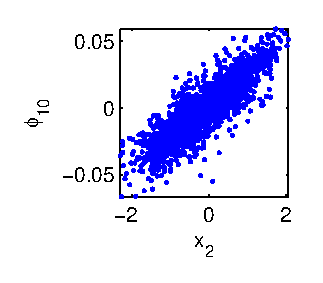
\epsfig{width=0.3\textwidth, file=data_linear_fast2.eps}
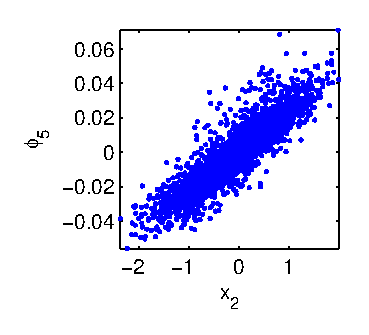
\epsfig{width=0.3\textwidth, file=data_linear_fast3.eps}

\epsfig{width=0.3\textwidth, file=data_linear_evals1.eps}
\epsfig{width=0.3\textwidth, file=data_linear_evals2.eps}
\epsfig{width=0.3\textwidth, file=data_linear_evals3.eps}

\caption{Relationship between changing $\delta t$ and recovery of the variables. From left to right, the columns correspond to $\delta t = 10^{-6}, 10^{-5}, 10^{-3}$.  (Row 1) Data (gray) and representative burst (red) used to estimate the local covariance. (Row 2) Correlation between first diffusion maps coordinate and the slow variable $x_1$. (Row 3) Correlation between diffusion maps coordinate and the fast variable $x_2$. Note that for $\delta t = 10^{-6}, 10^{-5}$, $x_2$ is correlated with $\phi_{10}$, whereas when $\delta t = 10^{-3}$, $x_2$ is correlated with $\phi_6$. (Row 4) Diffusion maps eigenvalue spectra. The eigenvalues corresponding to the coordinates for the fast and slow modes are indicated by red circles. }
\label{fig:recover_fast}
\end{figure}

\subsection{Nonlinear functions} \label{subsec:nonlinear_example}

In the second example, our data will be warped into half-moon shapes via the function 
\begin{equation} \label{eq:nonlinear_function}
\begin{aligned}
\begin{bmatrix}
y_1 \\ y_2
\end{bmatrix} &=&
\mathbf{f}(\vec{x}) &=& 
\begin{bmatrix} 
x_1 + x_2^2 \\
x_2
\end{bmatrix}\\
\mathbf{g}(\vec{y}) &=& \mathbf{f}^{-1} (\vec{y}) &=& \begin{bmatrix} y_1 - y_2^2 \\ y_2 \end{bmatrix}
\end{aligned}
\end{equation}
%
Figure~\ref{fig:initial_data_nonlinear} shows the data from Figure~\ref{fig:initial_data} transformed by the function $\mathbf{f}$ and colored by time. 

For this example, the analytical covariance is 
\begin{equation}
\begin{aligned}
C(\vec{x}) &=&
 \begin{bmatrix}
1+ \frac{4 x_2^2}{\epsilon} & \frac{2 x_2}{\epsilon} \\
\frac{2 x_2}{\epsilon} & \frac{1}{\epsilon} 
\end{bmatrix}\\
C^{\dagger}(\vec{x}) &=& 
\begin{bmatrix}
1 & -2 x_2 \\
-2 x_2 & \epsilon+ 4 x_2^2
\end{bmatrix} 
\end{aligned}
\end{equation}

\begin{figure}[t]
\centering
\epsfig{width=0.5\textwidth, file=data_init_nonlinear.eps}
\caption{The data from Figure~\ref{fig:initial_data}, transformed by $\mathbf{f}$ in \eqref{eq:nonlinear_function}}
\label{fig:initial_data_nonlinear}
\end{figure}

\begin{figure}[t]

\epsfig{width=0.5\textwidth, file=data_nonlinear_NIV_dt1_kernel1.eps}
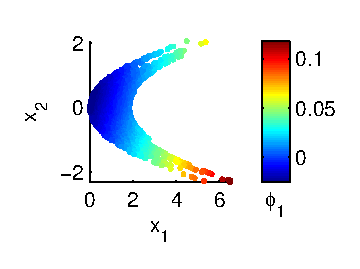
\epsfig{width=0.5\textwidth, file=data_nonlinear_DMAPS.eps}

\epsfig{width=0.5\textwidth, file=data_nonlinear_NIV_dt1_kernel2.eps}
\epsfig{width=0.5\textwidth, file=data_nonlinear_NIV_dt2_kernel1.eps}

\caption{(a) Data from Figure~\ref{fig:initial_data_nonlinear}, colored by the first DMAPS variable using the Mahalanobis distance with $\delta t = 10^{-7}$ and $\sigma_{kernel}^2 = 10^{-2}$. Note that the parameterization is one-to-one with the slow variable. (b) Data from Figure~\ref{fig:initial_data_nonlinear}, colored by the first DMAPS variable using the Euclidean distance. We do not recover the slow variable, because the Eiclidean distance is not informative as to the dynamics of the data. (c) Data from Figure~\ref{fig:initial_data_nonlinear}, colored by the first DMAPS variable using the Mahalanobis distance with $\delta t = 10^{-7}$ and $\sigma_{kernel}^2 = 10^{1}$. We do not recover the slow variable because $\sigma_{kernel}$ is too large. (d) Data from Figure~\ref{fig:initial_data_nonlinear}, colored by the first DMAPS variable using the Mahalanobis distance with $\delta t = 10^{-3}$ and $\sigma_{kernel}^2 = 10^{-2}$. We do not recover the slow variable because $\delta t$ is too large.  }
\label{fig:colored_data_nonlinear_cases}
\end{figure}

\subsubsection{Errors in Mahalanobis distance}

From \eqref{eq:distance_taylor_expansion}, we have 
\begin{equation}
e_M(\vec{y}_1, \vec{y}_2) = - (y_{2,2} - y_{1,2})^4 
+ \mathcal{O} (\|\vec{y}_1 - \vec{y}_2 \|^6 ) 
\end{equation}
%
We can bound the Mahalanobis distance by the eigenvalues of $C^{\dagger}$, 
\begin{equation}
\lambda_1 (C^{\dagger}) \| \vec{y}_2 - \vec{y}_1 \|^2 
\le 
(\vec{y}_2 - \vec{y}_1) C^{\dagger} (\vec{y}_2 - \vec{y}_1) 
\le 
\lambda_2 (C^{\dagger}) \| \vec{y}_2 - \vec{y}_1 \|^2  
\end{equation}
where $\lambda_1 (C^{\dagger}) \le \lambda_2 (C^{\dagger})$ are the two eigenvalues of $C^{\dagger}$. 

Figure~\ref{fig:cov_error_nonlinear}(a) shows $\| \vec{y}_2 - \vec{y}_1 \|^2_M$ and $e_M$ as a function of $\| \vec{y}_2 - \vec{y}_1 \|_2$. 
%
The Mahalanobis distance is an accurate approximation to the true intrinsic distance $\| \vec{z}_2 - \vec{z}_1 \|_2$ when $e_M \ll \| \vec{y}_2 - \vec{y}_1 \|^2_M$. 
%
We want to choose $\sigma_{kernel}^2$ in a regime where $e_M \ll \| \vec{y}_2 - \vec{y}_1 \|^2_M$, so that the distances we utilize in the diffusion maps calculation are accurate. 

We can find such a regime empirically by plotting $\| \vec{y}_2 - \vec{y}_1 \|^2_M$ as a function of $\| \vec{y}_2 - \vec{y}_1 \|_2$, and assessing when the relationship deviates from quadratic. 
%
This is shown in Figure~\ref{fig:cov_error_nonlinear}(b). 

Figures~\ref{fig:colored_data_nonlinear_cases}(a) and (c) show the data from Figure~\ref{fig:initial_data_nonlinear}, colored by $\phi_1$ for two different values of $\sigma_{kernel}$. 
%
The corresponding values of $\sigma_{kernel}^2$ are indicated by the dashed lines in Figure~\ref{fig:cov_error_nonlinear}(a)~and~(b). 
%
When $\sigma_{kernel}^2$ corresponds to a region where $\|e_M \| \ll \|\vec{y}_2 - \vec{y}_1 \|_M^2$, $\phi_1$ is well correlated with the slow variable.
%
However, when $\sigma_{kernel}^2$ corresponds to a region where $\|e_M \| \gg \|\vec{y}_2 - \vec{y}_1 \|_M^2$, the slow variable is no longer recovered. 

\subsubsection{Errors in covariance estimation}

From \eqref{eq:estimated_cov}, we find that
%
\begin{equation}
\begin{aligned}
e_{C, 11}(\vec{x}_t, \delta t) =& \frac{4}{\delta t \epsilon^{3/2}} \left( \sqrt{\epsilon} \mathbb{E} \left[ \left( \int_t^{t + \delta t} dW_{s,1} \right) \left( \int_t^{t+\delta t} \int_t^{s_2}  dW_{s_1, 2} dW_{s_2, 2} \right) \right] \right. \\
& \left. + 2 x_{t,2} \mathbb{E} \left[ \left( \int_t^{t + \delta t} dW_{s,2} \right) \left( \int_t^{t+\delta t} \int_t^{s_2}  dW_{s_1, 2} dW_{s_2, 2} \right) \right] \right) + \mathcal{O}(\delta t) \\
e_{C, 12}(\vec{x}_t, \delta t) =& \frac{2}{\delta t \epsilon^{3/2}} \mathbb{E} \left[ \left( \int_t^{t + \delta t} dW_{s,2} \right) \left( \int_t^{t+\delta t} \int_t^{s_2} dW_{s_1, 2} dW_{s_2, 2} \right) \right] + \mathcal{O}(\delta t)\\
e_{C, 21}(\vec{x}_t, \delta t) =& \frac{2}{\delta t \epsilon^{3/2}} \mathbb{E} \left[ \left( \int_t^{t + \delta t} dW_{s,2} \right) \left( \int_t^{t+\delta t} \int_t^{s_2} dW_{s_1, 2} dW_{s_2, 2} \right) \right] + \mathcal{O}(\delta t)\\
e_{C, 22}(\vec{x}_t, \delta t) =& \mathcal{O}(\delta t)
\end{aligned}
\end{equation}

$\|C \|$ and $\| e_C\|$ are shown as a function of $\delta t$ in Figure~\ref{fig:cov_error_nonlinear}(c).
%
As in the previous example, we can find where $\| e_c \| \ll \| C \|$  by plotting $\| \hat{C} \|$ as a function of $\delta t $ and looking for a kink in the plot. 
%
These results are shown in Figure~\ref{fig:cov_error_nonlinear}(d). 

Figures~\ref{fig:colored_data_nonlinear_cases}(a) and (d) show the data from Figure~\ref{fig:initial_data_nonlinear}, colored by $\phi_1$ for two different values of $\delta t$. 
%
The corresponding values of $\delta t$ are indicated by the dashed lines in Figure~\ref{fig:cov_error_nonlinear}(c)~and~(d). 
%
When $\delta t$ corresponds to a region where $\|e_C \| \ll \|C \|$, the slow variable is recovered by the first DMAPS coordinate.
%
However, when $\delta t$ corresponds to a region where $\|e_C \| \gg \|C \|$, the slow variable is no longer recovered. 

\begin{figure}[h]

\epsfig{width=0.5\textwidth, file=dist_dy_analytical_nonlinear.eps}
\epsfig{width=0.5\textwidth, file=dist_dy_nonlinear.eps}

\epsfig{width=0.5\textwidth, file=C_dt_analytical_nonlinear.eps}
\epsfig{width=0.5\textwidth, file=C_dt_nonlinear.eps}

\caption{Errors in the Mahalanobis distance and the covariance estimation for the nonlinear example. (a) The analytical expressions for the contributions to the distance approximation as a function of $\| \vec{y}_2 - \vec{y}_1\|_2$. (b) The average estimated Mahalanobis distance $\| \vec{y}_2 - \vec{y}_1\|^2_M$ as a function of the distance $\| \vec{y}_2 - \vec{y}_1\|_2$. The line $\| \vec{y}_2 - \vec{y}_1\|^2_M = \| \vec{y}_2 - \vec{y}_1\|_2$ is shown for reference. (c) The analytical expressions for the contributions to the covariance as a function of $\delta t$. (d) The average estimated covariance $\| \hat{C} \|$ as a function of $\delta t$. }
\label{fig:cov_error_nonlinear}
\end{figure}

\section{Conclusion}

We showed that in certain cases (when we do {\em not} have a simulator where we can change $\delta t$), the data cannot be processed as-is (we cannot find the right kernel scale given a fixed $\delta t$ such that we can accurately recover the slow variable). 

If the cloud of samples is too big then we can observe the cloud of clouds (and those clouds can be histograms, Fourier, scattering, etc.) as a way to get smaller clouds. 


Richardson extrapolation could allow us to get an estimate of a second-order term in the covariance estimation, thereby locally approximating the function using a quadratic form, rather than a linear form,  which can lead to a better/improved/more accurate ``Mahalanobis'' metric. 


\appendix 

\section{Local Invariant Metrics}

We have \eqref{eq:general_SDE}
\begin{equation}
\begin{aligned}
dx_i &= a_i(\vec{x}) dt + dW_i, & \: 1 \le i \le m \\
dx_i &= \frac{a_i(\vec{x})}{\epsilon} dt + \frac{1}{\sqrt{\epsilon}} dW_i , & \: m+1 \le i \le n
\end{aligned}
\end{equation}
%
We then use \eqref{eq:general_rescale}, to obtain
%
\begin{equation}
\begin{aligned}
d z_i &= a_i(\vec{z}) dt + dW_i, & \: 1 \le i \le m \\
d \frac{z_i}{\sqrt{\epsilon}} &= \frac{a_i(\vec{z})}{\epsilon} dt + \frac{1}{\sqrt{\epsilon}} dW_i , & \: m+1 \le i \le n
\end{aligned}
\end{equation}
%
which reduces to
%
\begin{equation}
\begin{aligned}
d z_i &= a_i(\vec{z}) dt + dW_i, & \: 1 \le i \le m \\
d z_i &= \frac{a_i(\vec{z})}{\sqrt{\epsilon}} dt + dW_i , & \: m+1 \le i \le n
\end{aligned}
\end{equation}

\section{Analysis}

\subsection{Error analysis of the Mahalanobis distance}

By Taylor expansion around $\vec{y}_1$,
%
\begin{equation}
\begin{aligned}
g_i(\vec{y}_2) =& 
g_i(\vec{y}_1) + \sum_{j=1}^d \left. \frac{\partial g_i}{\partial y_j} \right|_{\vec{y}_1} (y_{2,j}-y_{1,j})\\
&+ \frac{1}{2} \sum_{jk=1}^d \left. \frac{\partial^2 g_i}{\partial y_j} \right|_{\vec{y}_1} (y_{2,j}-y_{1,j}) (y_{2,k}-y_{1,k})\\
&+ \frac{1}{6} \sum_{jkl=1}^d \left. \frac{\partial^3 g_i}{\partial y_j \partial y_k \partial y_l} \right|_{\vec{y}_1} (y_{2,j}-y_{1,j}) (y_{2,k}-y_{1,k}) (y_{2,l}-y_{1,l}) \\
&+ \mathcal{O}( \|\vec{y}_2 - \vec{y}_1 \|^4)
\end{aligned}
\end{equation}
%
Multiplying through by $\sqrt{e_i}$ and
substituting in relationships from \eqref{eq:variable_rescaling}, we obtain
%
\begin{equation}
\begin{aligned}
z_{2,i} =& 
z_{1,i} + \sqrt{e_i} \sum_{j=1}^d \left. \frac{\partial g_i}{\partial y_j} \right|_{\vec{y}_1} (y_{2,j}-y_{1,j})\\
&+ \frac{\sqrt{e_i}}{2} \sum_{jk=1}^d \left. \frac{\partial^2 g_i}{\partial y_j \partial y_k} \right|_{\vec{y}_1} (y_{2,j}-y_{1,j}) (y_{2,k}-y_{1,k})\\
&+ \frac{\sqrt{e_i}}{6} \sum_{jkl=1}^d \left. \frac{\partial^3 g_i}{\partial y_j \partial y_k \partial y_l} \right|_{\vec{y}_1} (y_{2,j}-y_{1,j}) (y_{2,k}-y_{1,k}) (y_{2,l}-y_{1,l}) \\
&+ \mathcal{O}( \sqrt{e_i} \|\vec{y}_2 - \vec{y}_1 \|^4)
\end{aligned}
\end{equation}
%
Therefore, 
%
\begin{equation}
\begin{aligned}
& (z_{2,i} - z_{1,i})^2 = \\ 
& \left( \sqrt{e_i} \sum_{j=1}^d \left. \frac{\partial g_i}{\partial y_j} \right|_{\vec{y}_1} (y_{2,j}-y_{1,j}) \right) \left( \sqrt{e_i} \sum_{j=1}^d \left. \frac{\partial g_i}{\partial y_j} \right|_{\vec{y}_1} (y_{2,j}-y_{1,j}) \right) \\
&+ 2 \left( \sqrt{e_i} \sum_{j=1}^d \left. \frac{\partial g_i}{\partial y_j} \right|_{\vec{y}_1} (y_{2,j}-y_{1,j}) \right) \left( \frac{\sqrt{e_i}}{2} \sum_{jk=1}^d \left. \frac{\partial^2 g_i}{\partial y_j \partial y_k} \right|_{\vec{y}_1} (y_{2,j}-y_{1,j}) (y_{2,k}-y_{1,k}) \right) \\
&+ 2 \left( \sqrt{e_i} \sum_{j=1}^d \left. \frac{\partial g_i}{\partial y_j} \right|_{\vec{y}_1} (y_{2,j}-y_{1,j}) \right) \left( \frac{\sqrt{e_i}}{6} \sum_{jkl=1}^d \left. \frac{\partial^3 g_i}{\partial y_j \partial y_k \partial y_l} \right|_{\vec{y}_1} (y_{2,j}-y_{1,j}) (y_{2,k}-y_{1,k}) (y_{2,l}-y_{1,l}) \right) \\
&+ \left( \frac{\sqrt{e_i}}{2} \sum_{jk=1}^d \left. \frac{\partial^2 g_i}{\partial y_j \partial y_k} \right|_{\vec{y}_1} (y_{2,j}-y_{1,j}) (y_{2,k}-y_{1,k}) \right) \left( \frac{\sqrt{e_i}}{2} \sum_{jk=1}^d \left. \frac{\partial^2 g_i}{\partial y_j \partial y_k} \right|_{\vec{y}_1} (y_{2,j}-y_{1,j}) (y_{2,k}-y_{1,k}) \right) \\
&+ \mathcal{O}( e_i \|\vec{y}_2 - \vec{y}_1 \|^5) \\
=& e_i \sum_{jk=1}^d \left. \frac{\partial g_i}{\partial y_j} \right|_{\vec{y}_1} \left. \frac{\partial g_i}{\partial y_k} \right|_{\vec{y}_1} (y_{2,j}-y_{1,j}) (y_{2,k}-y_{1,k}) \\
&+ e_i \sum_{jkl=1}^d \left. \frac{\partial g_i}{\partial y_j} \right|_{\vec{y}_1} \left. \frac{\partial^2 g_i}{\partial y_k \partial y_l} \right|_{\vec{y}_1} (y_{2,j}-y_{1,j})  (y_{2,k}-y_{1,k}) (y_{2,l}-y_{1,l}) \\
&+ \frac{e_i}{3} \sum_{jklm=1}^d \left. \frac{\partial g_i}{\partial y_j} \right|_{\vec{y}_1} \left. \frac{\partial^3 g_i}{ \partial y_k \partial y_l \partial y_m} \right|_{\vec{y}_1} (y_{2,j}-y_{1,j}) (y_{2,k}-y_{1,k}) (y_{2,l}-y_{1,l})(y_{2,m}-y_{1,m}) \\
&+ \frac{e_i}{4} \sum_{jklm=1}^d \left. \frac{\partial^2 g_i}{\partial y_j \partial y_k} \right|_{\vec{y}_1} \left. \frac{\partial^2 g_i}{\partial y_l \partial y_m} \right|_{\vec{y}_1} (y_{2,j}-y_{1,j}) (y_{2,k}-y_{1,k}) (y_{2,l}-y_{1,l}) (y_{2,m}-y_{1,m}) \\
&+ \mathcal{O}(e_i \|\vec{y}_2 - \vec{y}_1 \|^5)
\end{aligned}
\end{equation}
%
and so the norm is
%
\begin{equation} \label{eq:appendix_z_norm}
\begin{aligned}
\|\vec{z}_2 - \vec{z}_1\|_2^2 =& 
\sum_{i=1}^n (z_{2,i} - z_{1,i})^2 \\
=& \sum_{i=1}^n e_i \sum_{jk=1}^d \left. \frac{\partial g_i}{\partial y_j} \right|_{\vec{y}_1} \left. \frac{\partial g_i}{\partial y_k} \right|_{\vec{y}_1} (y_{2,j}-y_{1,j}) (y_{2,k}-y_{1,k}) \\
&+ \sum_{i=1}^n e_i \sum_{jkl=1}^d \left. \frac{\partial g_i}{\partial y_j} \right|_{\vec{y}_1} \left. \frac{\partial^2 g_i}{\partial y_k \partial y_l} \right|_{\vec{y}_1} (y_{2,j}-y_{1,j})  (y_{2,k}-y_{1,k}) (y_{2,l}-y_{1,l}) \\
&+ \sum_{i=1}^n \frac{e_i}{3} \sum_{jklm=1}^d \left. \frac{\partial g_i}{\partial y_j} \right|_{\vec{y}_1} \left. \frac{\partial^3 g_i}{ \partial y_k \partial y_l \partial y_m} \right|_{\vec{y}_1} (y_{2,j}-y_{1,j}) (y_{2,k}-y_{1,k}) (y_{2,l}-y_{1,l})(y_{2,m}-y_{1,m}) \\
&+ \sum_{i=1}^n \frac{e_i}{4} \sum_{jklm=1}^d \left. \frac{\partial^2 g_i}{\partial y_j \partial y_k} \right|_{\vec{y}_1} \left. \frac{\partial^2 g_i}{\partial y_l \partial y_m} \right|_{\vec{y}_1} (y_{2,j}-y_{1,j}) (y_{2,k}-y_{1,k}) (y_{2,l}-y_{1,l}) (y_{2,m}-y_{1,m}) \\
&+ \sum_{i=1}^n \mathcal{O}( e_i \|\vec{y}_2 - \vec{y}_1 \|^5)
\end{aligned}
\end{equation}
%
We can write $\sum_{i=1}^n \mathcal{O}( e_i \|\vec{y}_2 - \vec{y}_1 \|^5) = \mathcal{O}( (m + (n-m) \epsilon) \|\vec{y}_2 - \vec{y}_1 \|^5) \approx \mathcal{O}( m \|\vec{y}_2 - \vec{y}_1 \|^5)$ for $\epsilon \ll 1$. 

We note that \eqref{eq:appendix_z_norm} is for expansion around $\vec{y}_1$. 
%
We can average expansions around $\vec{y}_1$ and $\vec{y}_2$ to gain one order of accuracy. 
%
\begin{equation} 
\begin{aligned}
& \|\vec{z}_2 - \vec{z}_1\|_2^2 \\
=& \frac{1}{2} \left( \|\vec{z}_2 - \vec{z}_1\|_{2, \text{expanded at } \vec{y}_1}^2  + \|\vec{z}_2 - \vec{z}_1\|_{2, \text{expanded at } \vec{y}_2}^2 \right) \\
=& \frac{1}{2} \sum_{i=1}^n e_i \sum_{jk=1}^d \left( \left. \frac{\partial g_i}{\partial y_j} \right|_{\vec{y}_1} \left. \frac{\partial g_i}{\partial y_k} \right|_{\vec{y}_1} + \left. \frac{\partial g_i}{\partial y_j} \right|_{\vec{y}_2} \left. \frac{\partial g_i}{\partial y_k} \right|_{\vec{y}_2} \right) (y_{2,j}-y_{1,j}) (y_{2,k}-y_{1,k}) \\
&+ \frac{1}{2} \sum_{i=1}^n e_i \sum_{jkl=1}^d \left( \left. \frac{\partial g_i}{\partial y_j} \right|_{\vec{y}_1} \left. \frac{\partial^2 g_i}{\partial y_k \partial y_l} \right|_{\vec{y}_1} - \left. \frac{\partial g_i}{\partial y_j} \right|_{\vec{y}_2} \left. \frac{\partial^2 g_i}{\partial y_k \partial y_l} \right|_{\vec{y}_2} \right) (y_{2,j}-y_{1,j})  (y_{2,k}-y_{1,k}) (y_{2,l}-y_{1,l}) \\
&+ \frac{1}{6} \sum_{i=1}^n e_i \sum_{jklm=1}^d \left( \left. \frac{\partial g_i}{\partial y_j} \right|_{\vec{y}_1} \left. \frac{\partial^3 g_i}{ \partial y_k \partial y_l \partial y_m} \right|_{\vec{y}_1} + \left. \frac{\partial g_i}{\partial y_j} \right|_{\vec{y}_2} \left. \frac{\partial^3 g_i}{ \partial y_k \partial y_l \partial y_m} \right|_{\vec{y}_2} \right) (y_{2,j}-y_{1,j}) (y_{2,k}-y_{1,k}) (y_{2,l}-y_{1,l})(y_{2,m}-y_{1,m}) \\
&+ \frac{1}{8} \sum_{i=1}^n e_i \sum_{jklm=1}^d \left( \left. \frac{\partial^2 g_i}{\partial y_j \partial y_k} \right|_{\vec{y}_1} \left. \frac{\partial^2 g_i}{\partial y_l \partial y_m} \right|_{\vec{y}_1} + \left. \frac{\partial^2 g_i}{\partial y_j \partial y_k} \right|_{\vec{y}_2} \left. \frac{\partial^2 g_i}{\partial y_l \partial y_m} \right|_{\vec{y}_2} \right) (y_{2,j}-y_{1,j}) (y_{2,k}-y_{1,k}) (y_{2,l}-y_{1,l}) (y_{2,m}-y_{1,m}) \\
&+ \mathcal{O}(m \|\vec{y}_2 - \vec{y}_1 \|^6)
\end{aligned}
\end{equation}
%
noting that the fifth-order error terms involve {\em differences} of derivatives evaluated at $\vec{y}_1$ and $\vec{y}_2$, and we assume that these differences are $\mathcal{O} (\| \vec{y}_2 - \vec{y}_1 \|)$. 

\subsection{Error analysis of the covariance estimation}


(Taken from Kloeden, P. and Platen, E. (1995) Numerical Solution of Stochastic Differential Equations. New York: Springer.)

Again, our SDE is
\begin{equation}
x_{t + \delta t, i} = x_{t, i} + \int_{t}^{t + \delta t} \frac{a_i(\vec{x}_s)}{e_i} ds + \int_{t}^{t+\delta t} \frac{1}{\sqrt{e_i}} dW_{s, i}
\end{equation}
where $1 \le i \le n$. 
%
From page 182, equation 5.3, for a general function $f$
%
\begin{equation} \label{eq:appendix_ito_taylor_sum}
f(\vec{x}_{t+\delta t}) = \sum_{\alpha \in \mathcal{A}} I_\alpha[f_\alpha (\vec{x}_t)]_{t, t+\delta t} + \sum_{\alpha \in \mathcal{B}(\mathcal{A})} I_\alpha [f_\alpha(\cdot, \vec{x})]_{t, t+\delta t}
\end{equation}
where $\mathcal{A}$ is a hierarchical set. 
%
We take 
\begin{equation}
 A = \{ \alpha \in M : l(\alpha) \le 1 \} = \{ (j) : 0 \le j \le n \} \cup \{v \}
\end{equation}
%
Then, \eqref{eq:appendix_ito_taylor_sum} becomes
\begin{equation} 
f(\vec{x}_{t+\delta t}) = I_{v} [f_v(\vec{x}_t)]_{t, t+\delta t} + \sum_{j=0}^n I_{(j)} [f_{(j)}(\vec{x}_t)]_{t, t+\delta t} + \sum_{j=0}^n \sum_{k=0}^n I_{(j,k)} [f_{(j,k)} ( \vec{x} )]_{t, t+\delta t}
\end{equation}

We have that (page 169)
\begin{itemize}
\item $I_v [f(\cdot)]_{t, t + \delta t} = f(t) = \mathcal{O}(1)$
\item $I_{(0)} [f(\cdot)]_{t, t + \delta t} = \int_{t}^{t + \delta t} f(s) ds = \mathcal{O}(\delta t)$
\item $I_{(j)} [f(\cdot)]_{t, t + \delta t} = \int_{t}^{t + \delta t} f(s) dW_{s,j} = \mathcal{O}(\sqrt{\delta t})$, for $j \ge 1$
\item $I_{(0,0)} [f(\cdot)]_{t, t + \delta t} = \int_{t}^{t + \delta t} \int_{t}^{s_2} f(s_1) ds_1 ds_2 = \mathcal{O}(\delta t^2)$
\item $I_{(j,0)} [f(\cdot)]_{t, t + \delta t} = \int_{t}^{t + \delta t} \int_{t}^{s_2} f(s_1) dW_{s_1, j} ds_2 = \mathcal{O}(\delta t^{3/2})$, for $j \ge 1$
\item $I_{(0,k)} [f(\cdot)]_{t, t + \delta t} = \int_{t}^{t + \delta t} \int_{t}^{s_2} f(s_1) ds_1 dW_{s_2, k} = \mathcal{O}(\delta t^{3/2})$, for $k \ge 1$
\item $I_{(j,k)} [f(\cdot)]_{t, t + \delta t} = \int_{t}^{t + \delta t} \int_{t}^{s_2} f(s_1) dW_{s_1, j} dW_{s_2, k} = \mathcal{O}(\delta t)$, for $j, k \ge 1$
\end{itemize}

From page 177,
\begin{itemize}
\item $f_v = f$
\item $f_{(j)} = \frac{1}{\sqrt{e_j}} \frac{\partial f}{\partial x_j}$ for $j \ge 1$
\item $f_{(0)} = \sum_{j=1}^n \frac{a_j(\vec{x})}{e_j} \frac{\partial f}{\partial x_j} + \frac{1}{2}\sum_{j=1}^n \frac{1}{e_j} \frac{\partial^2 f}{\partial x_j^2}$
\item $f_{(j, k)} = \frac{1}{\sqrt{e_j e_k}} \frac{\partial^2 f}{\partial x_j \partial x_k}$ for $j,k \ge 1$
\item $f_{(j,0)} = \frac{1}{\sqrt{e_j}} \left( \sum_{k=1}^n \frac{\partial}{\partial x_j} \left( \frac{a_k(\vec{x})}{e_k} \frac{\partial f}{\partial x_k} \right) + \frac{1}{2 e_k} \frac{\partial^3 f}{\partial x_j \partial x_k^2} \right)$
\item $f_{(0, j)} = \frac{1}{\sqrt{e_j}} \sum_{k=1}^n \frac{a_k(\vec{x})}{e_k} \frac{\partial^2 f}{\partial x_j \partial x_k} +\frac{1}{2 e_k}  \frac{\partial^3 f}{\partial x_j \partial^2 x_k}$
\item $f_{(0,0)} = \sum_{j,k=1}^n \frac{a_j(\vec{x})}{e_j} \frac{\partial}{\partial x_j} \left( \frac{a_k(\vec{x})}{e_k} \frac{\partial f}{\partial x_k} \right) + \frac{1}{2 e_k}\frac{a_j(\vec{x})}{e_j} \frac{\partial^3 f}{\partial x_j \partial x_k^2} + \frac{1}{2 e_j} \frac{\partial}{\partial x_j^2} \left( \frac{a_k(\vec{x})}{e_k} \frac{\partial f}{\partial x_k} \right) + \frac{1}{4 e_j e_k} \frac{\partial^4 f}{\partial x_j^2 \partial x_k^2}$
\end{itemize}
%
Therefore, we have
%
\begin{equation} 
\begin{aligned}
f(\vec{x}_{t+\delta t}) =&
f(\vec{x}_t) \\
&+ \int_t^{t + \delta t} f_{(0)}(\vec{x}_t) ds
+ \int_t^{t + \delta t} f_{(j)}(\vec{x}_t) dW_{s,j} \\
&+ \int_t^{t+\delta t} \int_t^{s_2} f_{(0,0)}(\vec{x}_{s_1}) ds_1 ds_2 \\
&+ \sum_{j=1}^n \int_t^{t+\delta t} \int_t^{s_2} f_{(j,0)}(\vec{x}_{s_1}) dW_{s_1, j} ds_2 \\
&+ \sum_{j=1}^n \int_t^{t+\delta t} \int_t^{s_2} f_{(0,j)}(\vec{x}_{s_1}) ds_1 dW_{s_2, j} \\
&+ \sum_{j, k=1}^n \int_t^{t+\delta t} \int_t^{s_2} f_{(j,k)}(\vec{x}_{s_1}) dW_{s_1, j} dW_{s_2, k} 
\end{aligned}
\end{equation}
%
Rearranging the terms in order of importance/scale, we obtain
\begin{equation} 
\begin{aligned}
f(\vec{x}_{t+\delta t}) =&
f(\vec{x}_t) \\
&+ \sum_{j=1}^n f_{(j)}(\vec{x}_t) \int_t^{t + \delta t} dW_{s,j} \\
&+  f_{(0)}(\vec{x}_t) \int_t^{t + \delta t} ds
+ \sum_{j, k=1}^n \int_t^{t+\delta t} \int_t^{s_2} f_{(j,k)}(\vec{x}_{s_1}) dW_{s_1, j} dW_{s_2, k} \\
&+ \sum_{j=1}^n \int_t^{t+\delta t} \int_t^{s_2} f_{(j,0)}(\vec{x}_{s_1}) dW_{s_1, j} ds_2 
+ \sum_{j=1}^n \int_t^{t+\delta t} \int_t^{s_2} f_{(0,j)}(\vec{x}_{s_1}) ds_1 dW_{s_2, j} \\
&+ \int_t^{t+\delta t} \int_t^{s_2} f_{(0,0)}(\vec{x}_{s_1}) ds_1 ds_2 
\end{aligned}
\end{equation}

We then want to compute $\mathbb{E}[f_1(\vec{x}_{t + \delta t})f_2(\vec{x}_{t + \delta t})] - \mathbb{E}[f_1(\vec{x}_{t + \delta t})]\mathbb{E}[f_2(\vec{x}_{t + \delta t})]$.
%
We calculate
\begin{equation} 
\begin{aligned}
\mathbb{E} [f(\vec{x}_{t+\delta t})] =&
f(\vec{x}_t) \\
&+  f_{(0)}(\vec{x}_t) \delta t
+ \sum_{j, k=1}^n \mathbb{E} \left[ \int_t^{t+\delta t} \int_t^{s_2} f_{(j,k)}(\vec{x}_{s_1}) dW_{s_1, j} dW_{s_2, k} \right] \\
&+ \sum_{j=1}^n \mathbb{E} \left[ \int_t^{t+\delta t} \int_t^{s_2} f_{(j,0)}(\vec{x}_{s_1}) dW_{s_1, j} ds_2  \right]
+ \sum_{j=1}^n \mathbb{E} \left[  \int_t^{t+\delta t} \int_t^{s_2} f_{(0,j)}(\vec{x}_{s_1}) ds_1 dW_{s_2, j} \right] \\
&+ \mathbb{E} \left[ \int_t^{t+\delta t} \int_t^{s_2} f_{(0,0)}(\vec{x}_{s_1}) ds_1 ds_2  \right]
\end{aligned}
\end{equation}
%
\begin{equation}
\begin{aligned}
&\mathbb{E} [f_1(\vec{x}_{t+\delta t})] \mathbb{E} [f_2(\vec{x}_{t+\delta t})] \\
=&
f_1(\vec{x}_t) f_2(\vec{x}_t) \\
&+  f_1(\vec{x}_t)f_{2,(0)}(\vec{x}_t) \delta t
+ f_1(\vec{x}_t)\sum_{j, k=1}^n \mathbb{E} \left[ \int_t^{t+\delta t} \int_t^{s_2} f_{2,(j,k)}(\vec{x}_{s_1}) dW_{s_1, j} dW_{s_2, k} \right] \\
&+ f_1(\vec{x}_t)\sum_{j=1}^n \mathbb{E} \left[ \int_t^{t+\delta t} \int_t^{s_2} f_{2,(j,0)}(\vec{x}_{s_1}) dW_{s_1, j} ds_2  \right]\\
&+ f_1(\vec{x}_t) \sum_{j=1}^n \mathbb{E} \left[ \int_t^{t+\delta t} \int_t^{s_2} f_{2,(0,j)}(\vec{x}_{s_1}) ds_1 dW_{s_2, j} \right] \\
&+ f_1(\vec{x}_t) \mathbb{E} \left[ \int_t^{t+\delta t} \int_t^{s_2} f_{2,(0,0)}(\vec{x}_{s_1}) ds_1 ds_2  \right]\\
&+ f_{1,(0)}(\vec{x}_t) \delta t f_2(\vec{x}_t) \\
&+ f_{1,(0)}(\vec{x}_t) \delta t f_{2,(0)}(\vec{x}_t) \delta t
+ f_{1,(0)}(\vec{x}_t) \delta t \sum_{j, k=1}^n \mathbb{E} \left[ \int_t^{t+\delta t} \int_t^{s_2} f_{2,(j,k)}(\vec{x}_{s_1}) dW_{s_1, j} dW_{s_2, k} \right] \\
&+ f_2(\vec{x}_t) \sum_{j, k=1}^n \mathbb{E} \left[ \int_t^{t+\delta t} \int_t^{s_2} f_{1,(j,k)}(\vec{x}_{s_1}) dW_{s_1, j} dW_{s_2, k} \right] \\
&+ f_{2,(0)}(\vec{x}_t) \delta t \sum_{j, k=1}^n \mathbb{E} \left[ \int_t^{t+\delta t} \int_t^{s_2} f_{1,(j,k)}(\vec{x}_{s_1}) dW_{s_1, j} dW_{s_2, k} \right] \\
&+ \sum_{j, k, l, m =1}^n \mathbb{E} \left[ \int_t^{t+\delta t} \int_t^{s_2} f_{1,(j,k)}(\vec{x}_{s_1}) dW_{s_1, j} dW_{s_2, k} \right] \mathbb{E} \left[ \int_t^{t+\delta t} \int_t^{s_2} f_{2,(l,m)}(\vec{x}_{s_1}) dW_{s_1, l} dW_{s_2, m} \right] \\
&+ f_2(\vec{x}_t) \sum_{j=1}^n \mathbb{E} \left[ \int_t^{t+\delta t} \int_t^{s_2} f_{1,(j,0)}(\vec{x}_{s_1}) dW_{s_1, j} ds_2  \right]  \\
&+ f_2(\vec{x}_t) \sum_{j=1}^n \mathbb{E} \left[  \int_t^{t+\delta t} \int_t^{s_2} f_{1,(0,j)}(\vec{x}_{s_1}) ds_1 dW_{s_2, j} \right] \\
&+ f_2(\vec{x}_t )\mathbb{E} \left[ \int_t^{t+\delta t} \int_t^{s_2} f_{1,(0,0)}(\vec{x}_{s_1}) ds_1 ds_2  \right]\\
&+ \mathcal{O}(\delta t^{5/2})
\end{aligned}
\end{equation}
%
\begin{equation}
\begin{aligned}
&f_1(\vec{x}_{t + \delta t}) f_2(\vec{x}_{t + \delta t}) \\
=& 
f_1(\vec{x}_t) f_2(\vec{x}_t) 
+  f_1(\vec{x}_t) \sum_{j=1}^n f_{2,(j)}(\vec{x}_t) \int_t^{t + \delta t} dW_{s,j} \\
&+  f_1(\vec{x}_t) f_{2,(0)}(\vec{x}_t) \int_t^{t + \delta t} ds
+ f_1(\vec{x}_t) \sum_{j, k=1}^n \int_t^{t+\delta t} \int_t^{s_2} f_{2, (j,k)}(\vec{x}_{s_1}) dW_{s_1, j} dW_{s_2, k} \\
&+ f_1(\vec{x}_t) \sum_{j=1}^n \int_t^{t+\delta t} \int_t^{s_2} f_{2, (j,0)}(\vec{x}_{s_1}) dW_{s_1, j} ds_2 
+ f_1(\vec{x}_t) \sum_{j=1}^n \int_t^{t+\delta t} \int_t^{s_2} f_{2, (0,j)}(\vec{x}_{s_1}) ds_1 dW_{s_2, j} \\
&+ f_1(\vec{x}_t) \int_t^{t+\delta t} \int_t^{s_2} f_{2, (0,0)}(\vec{x}_{s_1}) ds_1 ds_2 
+ \left( \sum_{j=1}^n f_{1,(j)}(\vec{x}_t) \int_t^{t + \delta t} dW_{s,j} \right) f_2(\vec{x}_t) \\
&+ \left( \sum_{j=1}^n f_{1,(j)}(\vec{x}_t) \int_t^{t + \delta t} dW_{s,j} \right) \sum_{j=1}^n f_{2,(j)}(\vec{x}_t) \int_t^{t + \delta t} dW_{s,j} 
+  \left(\sum_{j=1}^n f_{1,(j)}(\vec{x}_t) \int_t^{t + \delta t} dW_{s,j} \right)f_{2,(0)}(\vec{x}_t) \int_t^{t + \delta t} ds \\
&+ \left(\sum_{j=1}^n f_{1,(j)}(\vec{x}_t) \int_t^{t + \delta t} dW_{s,j} \right) \sum_{j, k=1}^n \int_t^{t+\delta t} \int_t^{s_2} f_{2,(j,k)}(\vec{x}_{s_1}) dW_{s_1, j} dW_{s_2, k} \\
&+ \left(\sum_{j=1}^n f_{1,(j)}(\vec{x}_t) \int_t^{t + \delta t} dW_{s,j} \right)\sum_{j=1}^n \int_t^{t+\delta t} \int_t^{s_2} f_{2,(j,0)}(\vec{x}_{s_1}) dW_{s_1, j} ds_2 \\
&+ \left(\sum_{j=1}^n f_{1,(j)}(\vec{x}_t) \int_t^{t + \delta t} dW_{s,j} \right)\sum_{j=1}^n \int_t^{t+\delta t} \int_t^{s_2} f_{2,(0,j)}(\vec{x}_{s_1}) ds_1 dW_{s_2, j} \\
&+\left( f_{1,(0)}(\vec{x}_t) \int_t^{t + \delta t} ds \right) f_2(\vec{x}_t) 
+  \left( f_{1,(0)}(\vec{x}_t) \int_t^{t + \delta t} ds \right)\sum_{j=1}^n f_{2,(j)}(\vec{x}_t) \int_t^{t + \delta t} dW_{s,j} \\
&+  \left( f_{1,(0)}(\vec{x}_t) \int_t^{t + \delta t} ds \right)f_{2,(0)}(\vec{x}_t) \int_t^{t + \delta t} ds
+ \left( f_{1,(0)}(\vec{x}_t) \int_t^{t + \delta t} ds \right)\sum_{j, k=1}^n \int_t^{t+\delta t} \int_t^{s_2} f_{2,(j,k)}(\vec{x}_{s_1}) dW_{s_1, j} dW_{s_2, k} \\
&+\left( \sum_{j, k=1}^n \int_t^{t+\delta t} \int_t^{s_2} f_{1,(j,k)}(\vec{x}_{s_1}) dW_{s_1, j} dW_{s_2, k} \right) f_2(\vec{x}_t) \\
&+  \left( \sum_{j, k=1}^n \int_t^{t+\delta t} \int_t^{s_2} f_{1,(j,k)}(\vec{x}_{s_1}) dW_{s_1, j} dW_{s_2, k} \right) \sum_{j=1}^n f_{2,(j)}(\vec{x}_t) \int_t^{t + \delta t} dW_{s,j} \\
&+ \left( \sum_{j, k=1}^n \int_t^{t+\delta t} \int_t^{s_2} f_{1,(j,k)}(\vec{x}_{s_1}) dW_{s_1, j} dW_{s_2, k} \right) f_{2,(0)}(\vec{x}_t) \int_t^{t + \delta t} ds \\
&+ \left( \sum_{j, k=1}^n \int_t^{t+\delta t} \int_t^{s_2} f_{1,(j,k)}(\vec{x}_{s_1}) dW_{s_1, j} dW_{s_2, k} \right)\sum_{j, k=1}^n \int_t^{t+\delta t} \int_t^{s_2} f_{2,(j,k)}(\vec{x}_{s_1}) dW_{s_1, j} dW_{s_2, k} \\
&+ \left( \sum_{j=1}^n \int_t^{t+\delta t} \int_t^{s_2} f_{1,(j,0)}(\vec{x}_{s_1}) dW_{s_1, j} ds_2  \right) f_2(\vec{x}_t) \\
&+  \left( \sum_{j=1}^n \int_t^{t+\delta t} \int_t^{s_2} f_{1,(j,0)}(\vec{x}_{s_1}) dW_{s_1, j} ds_2  \right)\left( \sum_{j=1}^n f_{2,(j)}(\vec{x}_t) \int_t^{t + \delta t} dW_{s,j} \right)\\
&+ \left( \sum_{j=1}^n \int_t^{t+\delta t} \int_t^{s_2} f_{1,(0,j)}(\vec{x}_{s_1}) ds_1 dW_{s_2, j}  \right) f_2(\vec{x}_t) \\
&+  \left( \sum_{j=1}^n \int_t^{t+\delta t} \int_t^{s_2} f_{1,(0,j)}(\vec{x}_{s_1}) ds_1 dW_{s_2, j}  \right)\left( \sum_{j=1}^n f_{2,(j)}(\vec{x}_t) \int_t^{t + \delta t} dW_{s,j} \right) \\
&+ \left( \int_t^{t+\delta t} \int_t^{s_2} f_{1,(0,0)}(\vec{x}_{s_1}) ds_1 ds_2 \right) f_2(\vec{x}_t) \\
&+ \mathcal{O} (\delta t^{5/2})
\end{aligned}
\end{equation}
%
Taking expectations, and using independence, we obtain
%
\begin{equation}
\begin{aligned}
&\mathbb{E} \left[ f_1(\vec{x}_{t + \delta t}) f_2(\vec{x}_{t + \delta t}) \right] \\
=& 
f_1(\vec{x}_t) f_2(\vec{x}_t) \\
&+  f_1(\vec{x}_t) f_{2,(0)}(\vec{x}_t) \delta t
+ f_1(\vec{x}_t) \sum_{j, k=1}^n \mathbb{E} \left[ \int_t^{t+\delta t} \int_t^{s_2} f_{2, (j,k)}(\vec{x}_{s_1}) dW_{s_1, j} dW_{s_2, k} \right] \\
&+ f_1(\vec{x}_t) \sum_{j=1}^n \mathbb{E}  \left[ \int_t^{t+\delta t} \int_t^{s_2} f_{2, (j,0)}(\vec{x}_{s_1}) dW_{s_1, j} ds_2 \right] 
+ f_1(\vec{x}_t) \sum_{j=1}^n \mathbb{E} \left[ \int_t^{t+\delta t} \int_t^{s_2} f_{2, (0,j)}(\vec{x}_{s_1}) ds_1 dW_{s_2, j} \right] \\
&+ f_1(\vec{x}_t) \int_t^{t+\delta t} \mathbb{E} \left[ \int_t^{s_2} f_{2, (0,0)}(\vec{x}_{s_1}) ds_1 ds_2 \right]
+  \sum_{j=1}^n f_{1,(j)}(\vec{x}_t) f_{2,(j)}(\vec{x}_t) \mathbb{E} \left[ \left( \int_t^{t + \delta t} dW_{s,j} \right)^2 \right] \\
&+ \sum_{j,k,l=1}^n f_{1,(j)}(\vec{x}_t) \mathbb{E} \left[ \left( \int_t^{t + \delta t} dW_{s,j} \right) \left( \int_t^{t+\delta t} \int_t^{s_2} f_{2,(k,l)}(\vec{x}_{s_1}) dW_{s_1, k} dW_{s_2, l} \right) \right] \\
&+ \sum_{j,k=1}^n f_{1,(j)}(\vec{x}_t) \mathbb{E} \left[ \left( \int_t^{t + \delta t} dW_{s,j} \right)\left( \int_t^{t+\delta t} \int_t^{s_2} f_{2,(k,0)}(\vec{x}_{s_1}) dW_{s_1, k} ds_2 \right) \right]\\
&+ \sum_{j, k=1}^n f_{1,(j)}(\vec{x}_t) \mathbb{E} \left[ \left( \int_t^{t + \delta t} dW_{s,j} \right) \left( \int_t^{t+\delta t} \int_t^{s_2} f_{2,(0,k)}(\vec{x}_{s_1}) ds_1 dW_{s_2, k} \right) \right] \\
&+f_{1,(0)}(\vec{x}_t) f_2(\vec{x}_t) \delta t
+  f_{1,(0)}(\vec{x}_t)f_{2,(0)}(\vec{x}_t) \delta t^2
+  f_{1,(0)}(\vec{x}_t) \delta t \sum_{j, k=1}^n \mathbb{E} \left[ \int_t^{t+\delta t} \int_t^{s_2} f_{2,(j,k)}(\vec{x}_{s_1}) dW_{s_1, j} dW_{s_2, k} \right] \\
&+f_2(\vec{x}_t) \sum_{j, k=1}^n \mathbb{E} \left[ \int_t^{t+\delta t} \int_t^{s_2} f_{1,(j,k)}(\vec{x}_{s_1}) dW_{s_1, j} dW_{s_2, k} \right] \\
&+  \sum_{j, k, l=1}^n  f_{2,(l)}(\vec{x}_t)\mathbb{E} \left[ \left( \int_t^{t+\delta t} \int_t^{s_2} f_{1,(j,k)}(\vec{x}_{s_1}) dW_{s_1, j} dW_{s_2, k} \right) \left( \int_t^{t + \delta t} dW_{s,l} \right) \right] \\
&+ f_{2,(0)}(\vec{x}_t) \delta t  \sum_{j, k=1}^n \mathbb{E} \left[ \int_t^{t+\delta t} \int_t^{s_2} f_{1,(j,k)}(\vec{x}_{s_1}) dW_{s_1, j} dW_{s_2, k} \right]  \\
&+ \sum_{j, k, l, m=1}^n \mathbb{E} \left[ \left( \int_t^{t+\delta t} \int_t^{s_2} f_{1,(j,k)}(\vec{x}_{s_1}) dW_{s_1, j} dW_{s_2, k} \right) \left( \int_t^{t+\delta t} \int_t^{s_2} f_{2,(l,m)}(\vec{x}_{s_1}) dW_{s_1, l} dW_{s_2, m} \right) \right] \\
&+ f_2(\vec{x}_t) \sum_{j=1}^n \mathbb{E} \left[ \int_t^{t+\delta t} \int_t^{s_2} f_{1,(j,0)}(\vec{x}_{s_1}) dW_{s_1, j} ds_2  \right]  \\
&+  \sum_{j, k=1}^n f_{2,(k)}(\vec{x}_t) \mathbb{E} \left[ \left( \int_t^{t+\delta t} \int_t^{s_2} f_{1,(j,0)}(\vec{x}_{s_1}) dW_{s_1, j} ds_2  \right) \left( \int_t^{t + \delta t} dW_{s,k} \right) \right]\\
&+ f_2(\vec{x}_t)  \sum_{j=1}^n \mathbb{E} \left[ \int_t^{t+\delta t} \int_t^{s_2} f_{1,(0,j)}(\vec{x}_{s_1}) ds_1 dW_{s_2, j}  \right]  \\
&+   \sum_{j, k=1}^n  f_{2,(k)}(\vec{x}_t) \mathbb{E} \left[ \left( \int_t^{t+\delta t} \int_t^{s_2} f_{1,(0,j)}(\vec{x}_{s_1}) ds_1 dW_{s_2, j}  \right) \left(\int_t^{t + \delta t} dW_{s,k} \right) \right] \\
&+ f_2(\vec{x}_t) \mathbb{E} \left[ \int_t^{t+\delta t} \int_t^{s_2} f_{1,(0,0)}(\vec{x}_{s_1}) ds_1 ds_2 \right]  \\
&+ \mathcal{O} (\delta t^{5/2})
\end{aligned}
\end{equation}

Therefore, 
%
\begin{equation}
\begin{aligned}
&\mathbb{E} \left[ f_1(\vec{x}_{t + \delta t}) f_2(\vec{x}_{t + \delta t}) \right] 
- \mathbb{E} \left[ f_1(\vec{x}_{t + \delta t}) \right] \mathbb{E} \left[ f_2(\vec{x}_{t + \delta t}) \right] \\
=& 
 \sum_{j=1}^n f_{1,(j)}(\vec{x}_t) f_{2,(j)}(\vec{x}_t) \mathbb{E} \left[ \left( \int_t^{t + \delta t} dW_{s,j} \right)^2 \right] \\
&+ \sum_{j,k,l=1}^n f_{1,(j)}(\vec{x}_t) \mathbb{E} \left[ \left( \int_t^{t + \delta t} dW_{s,j} \right) \left( \int_t^{t+\delta t} \int_t^{s_2} f_{2,(k,l)}(\vec{x}_{s_1}) dW_{s_1, k} dW_{s_2, l} \right) \right] \\
&+ \sum_{j,k=1}^n f_{1,(j)}(\vec{x}_t) \mathbb{E} \left[ \left( \int_t^{t + \delta t} dW_{s,j} \right)\left( \int_t^{t+\delta t} \int_t^{s_2} f_{2,(k,0)}(\vec{x}_{s_1}) dW_{s_1, k} ds_2 \right) \right]\\
&+ \sum_{j, k=1}^n f_{1,(j)}(\vec{x}_t) \mathbb{E} \left[ \left( \int_t^{t + \delta t} dW_{s,j} \right) \left( \int_t^{t+\delta t} \int_t^{s_2} f_{2,(0,k)}(\vec{x}_{s_1}) ds_1 dW_{s_2, k} \right) \right] \\
&+  \sum_{j, k, l=1}^n  f_{2,(l)}(\vec{x}_t)\mathbb{E} \left[ \left( \int_t^{t+\delta t} \int_t^{s_2} f_{1,(j,k)}(\vec{x}_{s_1}) dW_{s_1, j} dW_{s_2, k} \right) \left( \int_t^{t + \delta t} dW_{s,l} \right) \right] \\
&+ \sum_{j, k, l, m=1}^n \mathbb{E} \left[ \left( \int_t^{t+\delta t} \int_t^{s_2} f_{1,(j,k)}(\vec{x}_{s_1}) dW_{s_1, j} dW_{s_2, k} \right) \left( \int_t^{t+\delta t} \int_t^{s_2} f_{2,(l,m)}(\vec{x}_{s_1}) dW_{s_1, l} dW_{s_2, m} \right) \right] \\
&- \sum_{j, k, l, m =1}^n \mathbb{E} \left[ \int_t^{t+\delta t} \int_t^{s_2} f_{1,(j,k)}(\vec{x}_{s_1}) dW_{s_1, j} dW_{s_2, k} \right] \mathbb{E} \left[ \int_t^{t+\delta t} \int_t^{s_2} f_{2,(l,m)}(\vec{x}_{s_1}) dW_{s_1, l} dW_{s_2, m} \right] \\
&+  \sum_{j, k=1}^n f_{2,(k)}(\vec{x}_t) \mathbb{E} \left[ \left( \int_t^{t+\delta t} \int_t^{s_2} f_{1,(j,0)}(\vec{x}_{s_1}) dW_{s_1, j} ds_2  \right) \left( \int_t^{t + \delta t} dW_{s,k} \right) \right]\\
&+   \sum_{j, k=1}^n  f_{2,(k)}(\vec{x}_t) \mathbb{E} \left[ \left( \int_t^{t+\delta t} \int_t^{s_2} f_{1,(0,j)}(\vec{x}_{s_1}) ds_1 dW_{s_2, j}  \right) \left(\int_t^{t + \delta t} dW_{s,k} \right) \right] \\
&+ \mathcal{O} (\delta t^{5/2})
\end{aligned}
\end{equation}

For the case when $f$ is nonlinear, we need only consider up to $\mathcal{O}(\delta t^{3/2})$ terms. 
\begin{equation}
\begin{aligned}
\mathbb{E} \left[ f_1(\vec{x}_{t + \delta t}) f_2(\vec{x}_{t + \delta t}) \right] 
-& \mathbb{E} \left[ f_1(\vec{x}_{t + \delta t}) \right] \mathbb{E} \left[ f_2(\vec{x}_{t + \delta t}) \right] \\
=& 
\sum_{j=1}^n f_{1,(j)}(\vec{x}_t) f_{2,(j)}(\vec{x}_t) \mathbb{E} \left[ \left( \int_t^{t + \delta t} dW_{s,j} \right)^2 \right] \\
&+ \sum_{j,k,l=1}^n f_{1,(j)}(\vec{x}_t) \mathbb{E} \left[ \left( \int_t^{t + \delta t} dW_{s,j} \right) \left( \int_t^{t+\delta t} \int_t^{s_2} f_{2,(k,l)}(\vec{x}_{s_1}) dW_{s_1, k} dW_{s_2, l} \right) \right] \\
&+  \sum_{j, k, l=1}^n  f_{2,(l)}(\vec{x}_t)\mathbb{E} \left[ \left( \int_t^{t+\delta t} \int_t^{s_2} f_{1,(j,k)}(\vec{x}_{s_1}) dW_{s_1, j} dW_{s_2, k} \right) \left( \int_t^{t + \delta t} dW_{s,l} \right) \right] \\
&+ \mathcal{O} (\delta t^2)
\end{aligned}
\end{equation}
%
We then substitute expressions for $f$ and its derivatives, and using $\mathbb{E} \left[ \left( \int_t^{t + \delta t} dW_s \right)^2 \right] = \delta t$, we obtain
\begin{equation}
\begin{aligned}
\mathbb{E} \left[ f_1(\vec{x}_{t + \delta t}) f_2(\vec{x}_{t + \delta t}) \right] 
-& \mathbb{E} \left[ f_1(\vec{x}_{t + \delta t}) \right] \mathbb{E} \left[ f_2(\vec{x}_{t + \delta t}) \right] \\
=& 
\sum_{j=1}^n  \frac{1}{e_j} \left. \frac{\partial f_1}{\partial x_j} \right|_{\vec{x}_t} \left. \frac{\partial f_2}{\partial x_j} \right|_{\vec{x}_t} \delta t \\
&+ \sum_{j,k,l=1}^n \frac{1}{\sqrt{e_j e_k e_l}} \left. \frac{\partial f_1}{\partial x_j} \right|_{\vec{x}_t} \mathbb{E} \left[ \left( \int_t^{t + \delta t} dW_{s,j} \right) \left( \int_t^{t+\delta t} \int_t^{s_2} \left. \frac{\partial^2 f_2}{\partial x_k \partial x_l} \right|_{\vec{x}_{s_1}} dW_{s_1, k} dW_{s_2, l} \right) \right] \\
&+ \sum_{j,k,l=1}^n \frac{1}{\sqrt{e_j e_k e_l}} \left. \frac{\partial f_2}{\partial x_j} \right|_{\vec{x}_t} \mathbb{E} \left[ \left( \int_t^{t + \delta t} dW_{s,j} \right) \left( \int_t^{t+\delta t} \int_t^{s_2} \left. \frac{\partial^2 f_1}{\partial x_k \partial x_l} \right|_{\vec{x}_{s_1}} dW_{s_1, k} dW_{s_2, l} \right) \right] \\
&+ \mathcal{O} (\delta t^2)
\end{aligned}
\end{equation}

For the case when $f$ is linear, $f_{(j,k)} = f_{(0,j)} = 0$, and so
\begin{equation}
\begin{aligned}
\mathbb{E} \left[ f_1(\vec{x}_{t + \delta t}) f_2(\vec{x}_{t + \delta t}) \right] 
-& \mathbb{E} \left[ f_1(\vec{x}_{t + \delta t}) \right] \mathbb{E} \left[ f_2(\vec{x}_{t + \delta t}) \right] \\
=& 
 \sum_{j=1}^n f_{1,(j)}(\vec{x}_t) f_{2,(j)}(\vec{x}_t) \mathbb{E} \left[ \left( \int_t^{t + \delta t} dW_{s,j} \right)^2 \right] \\
&+ \sum_{j,k=1}^n f_{1,(j)}(\vec{x}_t) \mathbb{E} \left[ \left( \int_t^{t + \delta t} dW_{s,j} \right)\left( \int_t^{t+\delta t} \int_t^{s_2} f_{2,(k,0)}(\vec{x}_{s_1}) dW_{s_1, k} ds_2 \right) \right]\\
&+  \sum_{j, k=1}^n f_{2,(k)}(\vec{x}_t) \mathbb{E} \left[ \left( \int_t^{t+\delta t} \int_t^{s_2} f_{1,(j,0)}(\vec{x}_{s_1}) dW_{s_1, j} ds_2  \right) \left( \int_t^{t + \delta t} dW_{s,k} \right) \right]\\
&+ \mathcal{O} (\delta t^{5/2})
\end{aligned}
\end{equation}
%
Substituting in expressions for $f$ and its derivatives, and using $\mathbb{E} \left[ \left( \int_t^{t + \delta t} dW_s \right)^2 \right] = \delta t$, we obtain
\begin{equation}
\begin{aligned}
\mathbb{E} \left[ f_1(\vec{x}_{t + \delta t}) f_2(\vec{x}_{t + \delta t}) \right] 
-& \mathbb{E} \left[ f_1(\vec{x}_{t + \delta t}) \right] \mathbb{E} \left[ f_2(\vec{x}_{t + \delta t}) \right] \\
=& 
\sum_{j=1}^n  \frac{1}{e_j} \left. \frac{\partial f_1}{\partial x_j} \right|_{\vec{x}_t} \left. \frac{\partial f_2}{\partial x_j} \right|_{\vec{x}_t} \delta t \\
&+ \sum_{j,k,l=1}^n \frac{1}{e_l \sqrt{e_j e_k}} \left. \frac{\partial f_1}{\partial x_j} \right|_{\vec{x}_t} \mathbb{E} \left[ \left( \int_t^{t + \delta t} dW_{s,j} \right)\left( \int_t^{t+\delta t} \int_t^{s_2}  \frac{\partial f_2}{\partial x_l} \left. \frac{\partial a_l(\vec{x})}{\partial x_k} \right|_{\vec{x}_{s_1}} dW_{s_1, k} ds_2 \right) \right]\\
&+ \sum_{j,k,l=1}^n \frac{1}{e_l \sqrt{e_j e_k}} \left. \frac{\partial f_2}{\partial x_j} \right|_{\vec{x}_t} \mathbb{E} \left[ \left( \int_t^{t + \delta t} dW_{s,j} \right)\left( \int_t^{t+\delta t} \int_t^{s_2}  \frac{\partial f_1}{\partial x_l} \left. \frac{\partial a_l(\vec{x})}{\partial x_k} \right|_{\vec{x}_{s_1}} dW_{s_1, k} ds_2 \right) \right]\\
&+ \mathcal{O} (\delta t^{5/2})
\end{aligned}
\end{equation}

\section{Results}

\subsection{Linear functions}

For the linear case, 
\begin{equation}
\begin{aligned}
e_{C, i_1 i_2}(\vec{x}_t, \delta t) 
=& \frac{1}{\delta t} \sum_{j,k,l=1}^n \frac{1}{e_l \sqrt{e_j e_k}} \frac{\partial f_{i_1}}{\partial x_j} \mathbb{E} \left[ \left( \int_t^{t + \delta t} dW_{s,j} \right)\left( \int_t^{t+\delta t} \int_t^{s_2}  \frac{\partial f_{i_2}}{\partial x_l} \left. \frac{\partial a_l(\vec{x})}{\partial x_k} \right|_{\vec{x}_{s_1}} dW_{s_1, k} ds_2 \right) \right]\\
&+ \frac{1}{\delta t} \sum_{j,k,l=1}^n \frac{1}{e_l \sqrt{e_j e_k}} \frac{\partial f_{i_2}}{\partial x_j}  \mathbb{E} \left[ \left( \int_t^{t + \delta t} dW_{s,j} \right)\left( \int_t^{t+\delta t} \int_t^{s_2}  \frac{\partial f_{i_1}}{\partial x_l} \left. \frac{\partial a_l(\vec{x})}{\partial x_k} \right|_{\vec{x}_{s_1}} dW_{s_1, k} ds_2 \right) \right]\\
&+ \mathcal{O} (\delta t^{3/2})
\end{aligned}
\end{equation}

For the example in Section~\ref{subsec:linear_example}, 
\begin{equation}
\begin{aligned}
\frac{\partial f_1}{\partial x_1} = \frac{\partial f_2}{\partial x_2} &=& 1 \\
\frac{\partial f_2}{\partial x_1} = \frac{\partial f_1}{\partial x_2} &=& 0 \\
\frac{\partial a_1}{\partial x_i} &=& 0 \\
\frac{\partial a_2}{\partial x_1} &=& 0 \\
\frac{\partial a_2}{\partial x_2} &=& -1
\end{aligned}
\end{equation}

Therefore, we need only consider $k=l=2$
%
\begin{equation}
\begin{aligned}
e_{C, i_1 i_2}(\vec{x}_t, \delta t) 
=& -\frac{1}{\delta t \epsilon^{3/2}} \sum_{j=1}^n \frac{1}{\sqrt{e_j}} \frac{\partial f_{i_1}}{\partial x_j} \mathbb{E} \left[ \left( \int_t^{t + \delta t} dW_{s,j} \right)\left( \int_t^{t+\delta t} \int_t^{s_2}  \frac{\partial f_{i_2}}{\partial x_2} dW_{s_1, 2} ds_2 \right) \right]\\
&- \frac{1}{\delta t \epsilon^{3/2}} \sum_{j=1}^n \frac{1}{\sqrt{e_j}} \frac{\partial f_{i_2}}{\partial x_j}  \mathbb{E} \left[ \left( \int_t^{t + \delta t} dW_{s,j} \right)\left( \int_t^{t+\delta t} \int_t^{s_2}  \frac{\partial f_{i_1}}{\partial x_2} dW_{s_1, 2} ds_2 \right) \right]\\
&+ \mathcal{O} (\delta t^{3/2})
\end{aligned}
\end{equation}
%
Reducing terms further results in
\begin{equation}
\begin{aligned}
e_{C, 11}(\vec{x}_t, \delta t) &=& \mathcal{O} (\delta t^{3/2}) \\
e_{C, 12}(\vec{x}_t, \delta t) &=&  -\frac{1}{\delta t \epsilon^{3/2}} \mathbb{E} \left[ \left( \int_t^{t + \delta t} dW_{s,1} \right)\left( \int_t^{t+\delta t} \int_t^{s_2}  dW_{s_1, 2} ds_2 \right) \right] + \mathcal{O} (\delta t^{3/2})\\
e_{C, 21}(\vec{x}_t, \delta t) &=& -\frac{1}{\delta t \epsilon^{3/2}} \mathbb{E} \left[ \left( \int_t^{t + \delta t} dW_{s,1} \right)\left( \int_t^{t+\delta t} \int_t^{s_2}  dW_{s_1, 2} ds_2 \right) \right] + \mathcal{O} (\delta t^{3/2})\\
e_{C, 22}(\vec{x}_t, \delta t) &=& -\frac{2}{\delta t \epsilon^2} \mathbb{E} \left[ \left( \int_t^{t + \delta t} dW_{s,2} \right)\left( \int_t^{t+\delta t} \int_t^{s_2}  dW_{s_1, 2} ds_2 \right) \right] + \mathcal{O} (\delta t^{3/2}) 
\end{aligned}
\end{equation}

\subsection{Nonlinear functions}

The error in the Mahalanobis distance is given by \begin{equation}
\begin{aligned}
e_M =& 
 \frac{1}{2} \sum_{i=1}^n \sum_{jkl=1}^{d} e_i \left( \left. \frac{\partial g_i}{\partial y_j} \right|_{\vec{y}_1} \left. \frac{\partial^2 g_i}{\partial y_k \partial y_l} \right|_{\vec{y}_1} - \left. \frac{\partial g_i}{\partial y_j} \right|_{\vec{y}_2} \left. \frac{\partial^2 g_i}{\partial y_k \partial y_l} \right|_{\vec{y}_2} \right) (y_{2,j} - y_{1,j})  (y_{2,k} - y_{1,k})(y_{2,l} - y_{1,l}) \\
& + \frac{1}{8} \sum_{i=1}^n \sum_{jklm=1}^d  e_i \left( \left. \frac{\partial^2 g_i}{\partial y_j \partial y_k} \right|_{\vec{y}_1} \left. \frac{\partial^2 g_i}{\partial y_l \partial y_m} \right|_{\vec{y}_1} + \left. \frac{\partial^2 g_i}{\partial y_j \partial y_k} \right|_{\vec{y}_2} \left. \frac{\partial^2 g_i}{\partial y_l \partial y_m} \right|_{\vec{y}_2} \right) (y_{2,j} - y_{1,j})  (y_{2,k} - y_{1,k})(y_{2,l} - y_{1,l})(y_{2,m} - y_{1,m}) \\
& + \frac{1}{6} \sum_{i=1}^n \sum_{jklm=1}^d e_i \left( \left. \frac{\partial g_i}{\partial y_j} \right|_{\vec{y}_1} \left. \frac{\partial^3 g_i}{ \partial y_k \partial y_l \partial y_m} \right|_{\vec{y}_1} + \left. \frac{\partial g_i}{\partial y_j} \right|_{\vec{y}_2} \left. \frac{\partial^3 g_i}{ \partial y_k \partial y_l \partial y_m} \right|_{\vec{y}_2} \right) (y_{2,j} - y_{1,j})  (y_{2,k} - y_{1,k})(y_{2,l} - y_{1,l})(y_{2,m} - y_{1,m}) \\
& + \mathcal{O} (\|\vec{y}_1 - \vec{y}_2 \|^6 )
\end{aligned}
\end{equation}

For our specific example in in Section~\ref{subsec:nonlinear_example}, 
\begin{equation}
\begin{aligned}
\frac{\partial g_1}{\partial y_1} = \frac{\partial g_2}{\partial y_2} &=& 1 \\
\frac{\partial g_1}{\partial y_2} &=& -2 y_2 \\
\frac{\partial g_2}{\partial y_1} &=& 0 \\
\frac{\partial^2 g_1}{\partial y_1^2} = \frac{\partial^2 g_1}{\partial y_1 \partial y_2} &=& 0 \\
\frac{\partial^2 g_1}{\partial y_2^2} &=& -2 \\
\frac{\partial^2 g_2}{\partial y_i \partial y_j} &=& 0 \\
\frac{\partial^3 g}{\partial y_i \partial y_j \partial y_k} &=& 0
\end{aligned}
\end{equation}
%
and therefore, 
\begin{equation}
e_M =
 -(y_{2,2} - y_{1,2})^4
 + \mathcal{O} (\|\vec{y}_1 - \vec{y}_2 \|^6 )
\end{equation}

The errors in the covariance are given by
\begin{equation}
\begin{aligned}
e_C 
=& 
\frac{1}{\delta t} \sum_{j,k,l=1}^n \frac{1}{\sqrt{e_j e_k e_l}} \left. \frac{\partial f_{i_1}}{\partial x_j} \right|_{\vec{x}_t} \mathbb{E} \left[ \left( \int_t^{t + \delta t} dW_{s,j} \right) \left( \int_t^{t+\delta t} \int_t^{s_2} \left. \frac{\partial^2 f_{i_2}}{\partial x_k \partial x_l} \right|_{\vec{x}_{s_1}} dW_{s_1, k} dW_{s_2, l} \right) \right] \\
&+ \frac{1}{\delta t}  \sum_{j,k,l=1}^n \frac{1}{\sqrt{e_j e_k e_l}} \left. \frac{\partial f_{i_2}}{\partial x_j} \right|_{\vec{x}_t} \mathbb{E} \left[ \left( \int_t^{t + \delta t} dW_{s,j} \right) \left( \int_t^{t+\delta t} \int_t^{s_2} \left. \frac{\partial^2 f_{i_1}}{\partial x_k \partial x_l} \right|_{\vec{x}_{s_1}} dW_{s_1, k} dW_{s_2, l} \right) \right] \\
&+ \mathcal{O} (\delta t)
\end{aligned}
\end{equation}
%
For our specific example in in Section~\ref{subsec:nonlinear_example}, 
\begin{equation}
\begin{aligned}
\frac{\partial f_1}{\partial x_1} = \frac{\partial f_2}{\partial x_2} &=& 1 \\
\frac{\partial f_1}{\partial x_2} &=& 2 x_2 \\
\frac{\partial f_2}{\partial x_1} &=& 0 \\
\frac{\partial^2 f_1}{\partial x_1^2} = \frac{\partial^2 f_1}{\partial x_1 \partial x_2} &=& 0 \\
\frac{\partial^2 f_1}{\partial x_2^2} &=& 2 \\
\frac{\partial^2 f_2}{\partial x_i \partial x_j} &=& 0 \\
\end{aligned}
\end{equation}
%
and therefore
\begin{equation}
\begin{aligned}
e_{C, 11}(\vec{x}_t, \delta t) =& \frac{4}{\delta t \epsilon^{3/2}} \left( \sqrt{\epsilon} \mathbb{E} \left[ \left( \int_t^{t + \delta t} dW_{s,1} \right) \left( \int_t^{t+\delta t} \int_t^{s_2}  dW_{s_1, 2} dW_{s_2, 2} \right) \right] \right. \\
& \left. + 2 x_{t,2} \mathbb{E} \left[ \left( \int_t^{t + \delta t} dW_{s,2} \right) \left( \int_t^{t+\delta t} \int_t^{s_2}  dW_{s_1, 2} dW_{s_2, 2} \right) \right] \right) + \mathcal{O}(\delta t) \\
e_{C, 12}(\vec{x}_t, \delta t) =& \frac{2}{\delta t \epsilon^{3/2}} \mathbb{E} \left[ \left( \int_t^{t + \delta t} dW_{s,2} \right) \left( \int_t^{t+\delta t} \int_t^{s_2} dW_{s_1, 2} dW_{s_2, 2} \right) \right] + \mathcal{O}(\delta t)\\
e_{C, 21}(\vec{x}_t, \delta t) =& \frac{2}{\delta t \epsilon^{3/2}} \mathbb{E} \left[ \left( \int_t^{t + \delta t} dW_{s,2} \right) \left( \int_t^{t+\delta t} \int_t^{s_2} dW_{s_1, 2} dW_{s_2, 2} \right) \right] + \mathcal{O}(\delta t)\\
e_{C, 22}(\vec{x}_t, \delta t) =& \mathcal{O}(\delta t)
\end{aligned}
\end{equation}
%


\end{document}
